%%%%%%%%%%%%%%%%%%%%%%%%%%%%%%%%%%%%%%%%%%%%%%%%%%%%%%%%%%%%%%%%%%%%%%%%%%%%%%%
% Neuroimage-like layout
\documentclass[5p]{elsarticle}
% For kindle
%\documentclass[1p,12pt]{elsarticle}
%\usepackage{geometry}
%\geometry{a6paper,hmargin={.2cm,.2cm},vmargin={1cm,1cm}}
% End kindle
\usepackage{amsmath,amsfonts,amssymb}
\usepackage{bm}
\usepackage{algorithm}
\usepackage{algorithmic}
\usepackage{url}
\usepackage[breaklinks=true,letterpaper=true,colorlinks,bookmarks=false]{hyperref}
\usepackage[table]{xcolor}

\definecolor{deep_blue}{rgb}{0,.2,.5}
\definecolor{dark_blue}{rgb}{0,.15,.5}

\hypersetup{pdftex,  % needed for pdflatex
  breaklinks=true,  % so long urls are correctly broken across lines
  colorlinks=true,
  linkcolor=dark_blue,
  citecolor=deep_blue,
}

% Float parameters, for more full pages.
\renewcommand{\topfraction}{0.9}        % max fraction of floats at top
\renewcommand{\bottomfraction}{0.8}     % max fraction of floats at bottom
\renewcommand{\textfraction}{0.07}      % allow minimal text w. figs
%   Parameters for FLOAT pages (not text pages):
\renewcommand{\floatpagefraction}{0.6}  % require fuller float pages
%    % N.B.: floatpagefraction MUST be less than topfraction !!


\def\B#1{\mathbf{#1}}
%\def\B#1{\bm{#1}}
\def\trans{^\mathsf{T}}
% A compact fraction
\def\slantfrac#1#2{\kern.1em^{#1}\kern-.1em/\kern-.1em_{#2}}

%%%%%%%%%%%%%%%%%%%%%%%%%%%%%%%%%%%%%%%%%%%%%%%%%%%%%%%%%%%%%%%%%%%%%%%%%%%%%%%%
\begin{document}

\title{Learning and comparing functional connectomes across subjects}


\author[parietal,unicog,cea]{Ga\"el Varoquaux\corref{corresponding}}
\author[cmi,nki]{R. Cameron Craddock}

\cortext[corresponding]{Corresponding author}

\address[parietal]{Parietal project-team, INRIA Saclay-\^ile de France}
\address[unicog]{INSERM, U992}
\address[cea]{CEA/Neurospin b\^at 145, 91191 Gif-Sur-Yvette}
\address[cmi]{Child Mind Institute, New York, New York}
\address[nki]{Nathan Kline Institute for Psychiatric Research, Orangeburg, New York}

\begin{abstract}
    Functional connectomes capture brain interactions via 
    fluctuations in brain imaging signal. On rest data they map
    the intrinsic functional architecture of the brain. With
    task-driven experiments they represent the integration mechanisms
    between specialized brain areas. Analysis of their variability 
    across subjects and conditions can reveal markers of brain
    pathologies and cognitive mechanisms. However, connectomes are
    complex multivariate objects. Methods to estimate them 
    from the functional signal have undergone rapid developments.
    The literature is full of diverse strategies to compare them.
    This paper aims to clarify some links across functional-connectivity
    methods and expose different steps to perform a group study on
    functional connectomes.
\end{abstract}

\begin{keyword}
    Functional connectivity, connectome, group study, effective
    connectivity, fMRI, resting-state
\end{keyword}

\maketitle
%%%%%%%%%%%%%%%%%%%%%%%%%%%%%%%%%%%%%%%%%%%%%%%%%%%%%%%%%%%%%%%%%%%%%%%%%%%%%%%%

\sloppy % Fed up with messed-up line breaks

\section{Introduction}

% General introduction
Functional connectivity reveals the synchronization of distant
neural systems via correlations in brain activity
\cite{biswal1995,friston1993}. Given that high-level
function emerges from the interaction of specialized units
\cite{tononi1992}, functional
connectivity is an essential part of the description of brain function,
that complements the localizationist picture emerging from the systematic
mapping of regions recruited in tasks \cite{sporns2005,biswal2010}. However, while there exists a
well-defined standard analysis framework for activation mapping that enables
statistically-controlled comparisons across subjects \cite{friston1995},
group-level analysis of functional connectivity still faces many open
methodological challenges. Deriving a picture of a single subject's 
functional connectivity is by itself not straightforward, as the brain
comprises a myriad of interacting subsystems and its connectivity must 
be decomposed into
simplified and synthetic representations. An important view of brain
connectivity is that of distributed functional networks depicted by their
spatial maps \cite{fox2005}. Another no less important and complementary
view is that of connections linking localized functional modules depicted
as a graph \cite{bullmore2009}. This representation of brain connectivity
is often called the functional connectome \cite{sporns2005} and is the
focus of intense worldwide research efforts as it holds promises of new
insights in cognition and pathologies
\cite{greicius2008b,biswal2010,fox2010}.

% Give the scope of the paper and narrow it
The purpose of this paper is to review methodological progress in the
estimation and comparison of functional connectomes. It does not attempt
to be exhaustive, as the field is wide and moving rapidly, but details
specific tools and guidelines that, in the experience of the authors,
lead to controlled and powerful inter-subject comparisons. The paper is
focused on functional connectomes in contrast to structural connectomes,
as the inference of functional connectivity from observed brain activity
fluctuations brings important specificities in the statistical modeling. While 
the notion of functional
connectome is often associated with the study of resting-state
\cite{biswal2010}, the methods presented in this paper are also relevant
for task-based studies. On the other hand, the paper has a focus on fMRI;
although the core concepts presented can be applied to MEG or EEG
\cite{stam2004}, additional specific problems such as source
reconstruction must be considered \cite{schoffelen2009}.

% Define terms
By ``functional connectome'', here we specifically denote a graph
representing functional interactions in the brain, where the term
``graph'' is taken in its mathematical sense: a set of \emph{nodes}
connected together by \emph{edges}. Nodes are localized functional units
and edges represent long range interactions synchronized via fibers.
A graph can be weighted or not, and
is completely equivalent to its \emph{adjacency matrix}, a symmetric
matrix tabulating the connection weights between each pair of nodes.
Functional-connectivity graphs are used to represent evoked activity,
as in task-response studies \cite{mcintosh2000}, as well as
ongoing activity, present in the absence of specific tasks or in 
the background during task and often studied in so-called \emph{resting-state}
experiments \cite{raichle2010}. Another important notion that arises from
the study of distributed modes of brain function is that of specialized
functional networks\footnote{In neuroimaging, the term network is
sometimes used to denote a graph of brain function. To disambiguate the
notion of segregated spatial mode \cite{fox2005} from that of
connectivity graphs, we will purposely restrict its usage in this
paper.} \cite{fox2005}. With our definition of the functional connectome, functional
networks are not directly building blocks of the connectome but appear
as a consequence of the graphical structure
\cite{varoquaux2010c,varoquaux2012}.

% Give a layout of the paper
The paper is organized as follows. First we discuss estimation of
functional connectomes. This part, akin to a first-level analysis in
standard activation mapping methodology, is not in itself a group-level
operation, but it is a critical step for inter-subject comparison.
In a following section, we discuss several strategies for comparing
connectomes across subjects. Finally we discuss the links between the
representation of brain connectivity as graphs of functional connectivity
and more complex models, such as effective-connectivity models.


%%%%%%%%%%%%%%%%%%%%%%%%%%%%%%%%%%%%%%%%%%%%%%%%%%%%%%%%%%%%%%%%%%%%%%%%%%%%%%%

\section{Estimating functional connectomes}

Here we discuss the inference of connectomes from functional brain
imaging data. We start with the choice of nodes \emph{i.e.}\ regions,
followed by signal extraction, and the estimation of graphs.

%------------------------------------------------------------------------------
\subsection{Defining regions}

The choice of regions of interests (ROIs) that define the nodes of the
graphs can be very important both in the estimation of connectomes and
for group comparison \cite{wang2009}. Unsurprisingly, simulations have
shown that extracting signal from ROIs that did not match functional
units would lead to erronous graph estimation \cite{smith2011}.
%
Different strategies to define suitable ROIs coexist. While dense parcellations approaches cover
a large fraction of the brain \cite{achard2006, varoquaux2010c,
wang2009,bellec2006}, this coverage can be traded off to focus on some specific
regions, in favor of increased functional specificity and thus better
differentiation across networks \cite{greicius2003, dosenbach2010,
varoquaux2010b}. In addition, while
ROIs are most often defined as a hard selection of voxels, it is also
possible to use a \emph{soft} definition, attributing weights as with
probabilistic atlases, or spatial maps of functional networks extracted
from techniques such as independent component analysis (ICA)
\cite{kiviniemi2009,smith2009}.

\paragraph{Regions from atlases}
%
Atlases can be used to define full-brain parcellations. A popular
is probably the AAL atlas \cite{tzourio-mazoyer2002a}, that
benefits from an SPM toolbox. However, it suffers from major
shortcomings; namely \emph{i)} that it was defined on a single subject
and thus does does not reflect inter-subject variability and \emph{ii)}
that it focuses on labeling large anatomical structures and does not match
functional layout \cite{craddock2011} --for instance only two regions describe the medial
part of the frontal lobe. Multi-subject probabilistic altases such as the
Harvard-Oxford atlas distributed with FSL \cite{smith2004} or the
sulci-based structural atlas used in \cite{varoquaux2010c} mitigate the
first problem, and the high number of regions defined using sulci also
somewhat circumvent the second problem (see
fig.\,\ref{fig:parcellations}).


\paragraph{Defining regions from the literature}
%
Regions can be defined from previous studies, informally or with
systematic meta-analysis. This strategy is used to define the main
resting-state networks, such as the default mode network, but may also be
useful to study connectivity in task-specific networks
\cite{biswal1995,rissman2004,grillon2012}. The common practice is to place balls of a given
radius, 5 or 10\,mm, centered at the coordinates of interest. Given that
functional networks are tightly interleaved in some parts of the cortex,
such as the parietal lobe, care must be taken not to define too many
regions that would overlap and lead to mixing of the signal.

\paragraph{FMRI-based function definition}
%
Defining regions directly from the fMRI signal brings many benefits.
First, it can capture subject-specific functional information. Second, it
adapts to the signal at hand and its limitations, such as
EPI-specific warps or vascular and movement artifacts that are isolated
in ICA-like approaches. The simplest approach to define task-specific
regions is to use activation maps derived from standard GLM-based
analysis in a task-driven study (see for instance \cite{poldrack2011}).
Regions are extracted by thresholding the maps, or using balls around the
activation peaks. For resting-state studies, unsupervised multivariate
analysis techniques are necessary. Clustering approaches extract
full-brain parcellations \cite{craddock2011, bellec2010, yeo2011,
thirion2006}, and have been shown to segment well-known functional
structures from rest data. Alternatively, decompositions
methods, such as ICA \cite{beckmann2004}, can unmix linear
combinations of multiple effects and separate out overlapping spatial maps
capturing functional networks or confounding effects. At high model
order, ICA maps define a functional parcellation \cite{kiviniemi2009}.
Extracting regions from these maps requires additional effort as they can
display fragmented spatial features and structured background noise, but
incorporating sparsity and spatial constraints in the decomposition
techniques leads to contrasted maps that outline many different
structures \cite{craddock2011, varoquaux2012} (see fig.\,\ref{fig:parcellations}).

%{{{------ Parcellation figure -----------------------------------------------
\begin{figure}
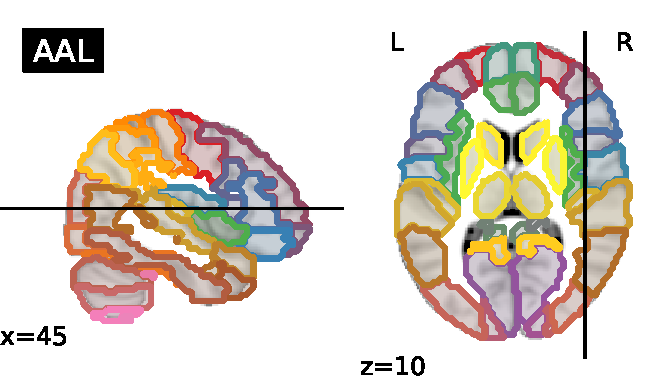
\includegraphics[width=.5\linewidth]{aal_atlas.pdf}%
\hfill%
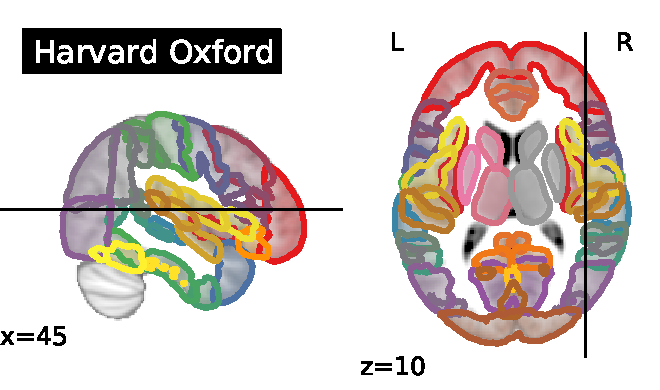
\includegraphics[width=.5\linewidth]{ho_atlas.pdf}%

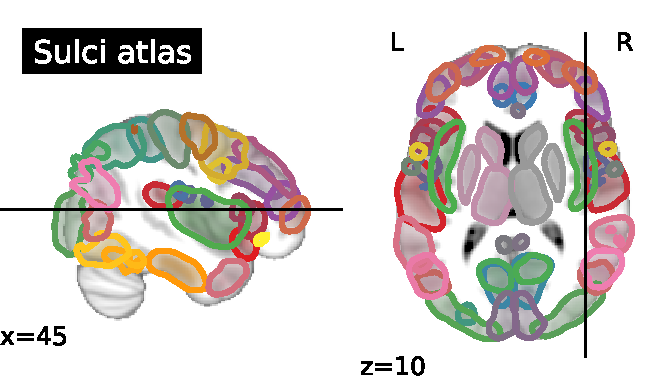
\includegraphics[width=.5\linewidth]{sulci_atlas.pdf}%
\hfill%
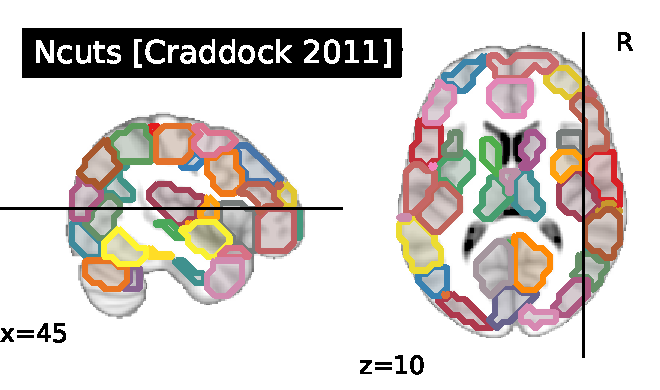
\includegraphics[width=.5\linewidth]{ncuts_atlas.pdf}%

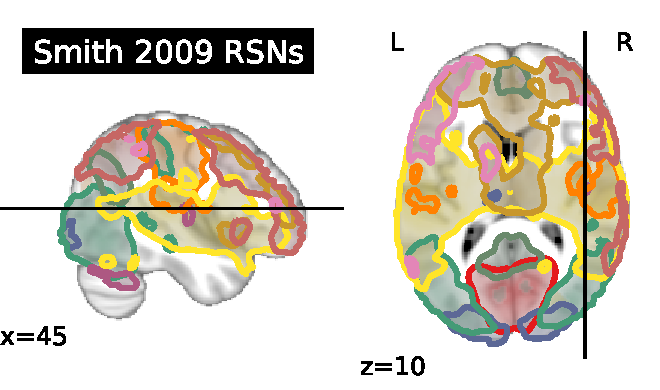
\includegraphics[width=.5\linewidth]{smith_atlas.pdf}%
\hfill%
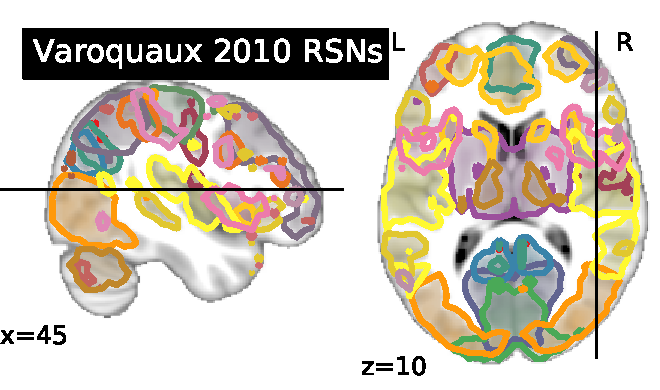
\includegraphics[width=.5\linewidth]{msdl_atlas.pdf}%

\caption{
Different full-brain parcellations: the AAL atlas
\cite{tzourio-mazoyer2002a}, the Harvard-Oxford atlas, the sucli atlas used in
\cite{varoquaux2010c}, regions extracted by Ncuts
\cite{craddock2011}, the resting-state networks extracted in
\cite{smith2009} by ICA, and in \cite{varoquaux2011} by sparse dictionary
learning.
\label{fig:parcellations}
}
\end{figure}
%---------------------------------------------------------------------------}}}

%------------------------------------------------------------------------------
\subsection{Estimating connections}

The concept of functional connectivity has be called elusive
\cite{horwitz2003}: it has many mathematical instantiations although in
essence they all strive to extract simple statistics from functional
imaging in order to characterize synchrony and communication between large
ensembles of neurons. Here we choose to focus on second order statistics
that can be related to Gaussian models, the simplest of which being the
correlation matrix of the signals of the different ROIs.


%{{{------ Correlation matrices figure ---------------------------------------
\begin{figure}
\newcommand{\photoframe}[1]{\setlength\fboxsep{0pt}%
{\color{black!70}\fbox{#1}\color{black}}}%
\begin{minipage}{.666\linewidth}%
    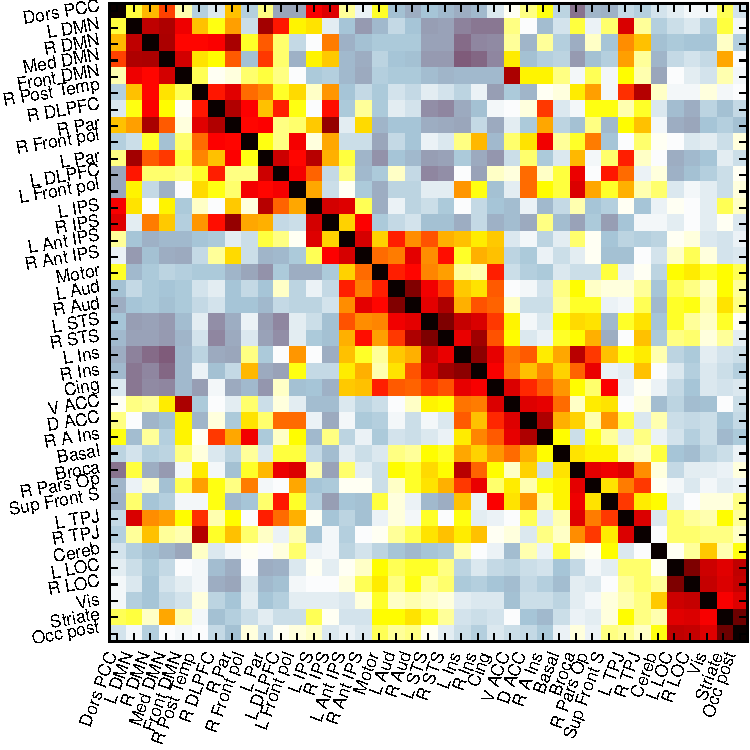
\includegraphics[width=\linewidth]{group_emp_cov.pdf}%
    \raisebox{.606\linewidth}{%
	\hspace*{-.462\linewidth}%
	\photoframe{%
	%\setlength\fboxsep{1pt}%
	\colorbox{white}{%
	\raisebox{.003\linewidth}{%
	    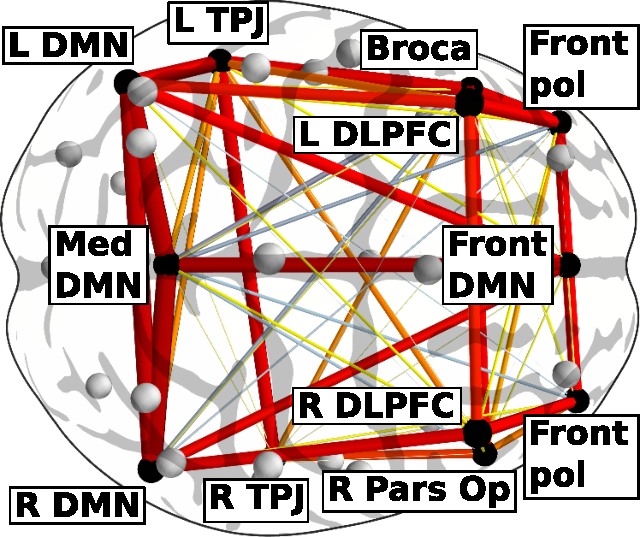
\includegraphics[width=.455\linewidth]{group_emp_cov_3d_labels}}%
	\rule{0pt}{.387\linewidth}%
	}}%
    }
\end{minipage}%
\hspace*{1pt}%
\begin{minipage}{.33\linewidth}%
    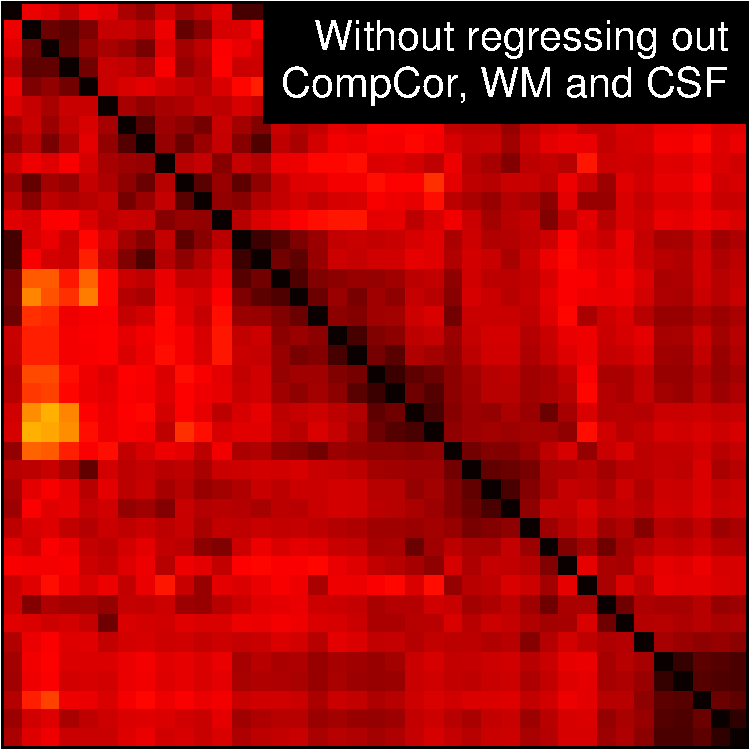
\includegraphics[width=\linewidth]{group_emp_cov_no_confounds.pdf}%

    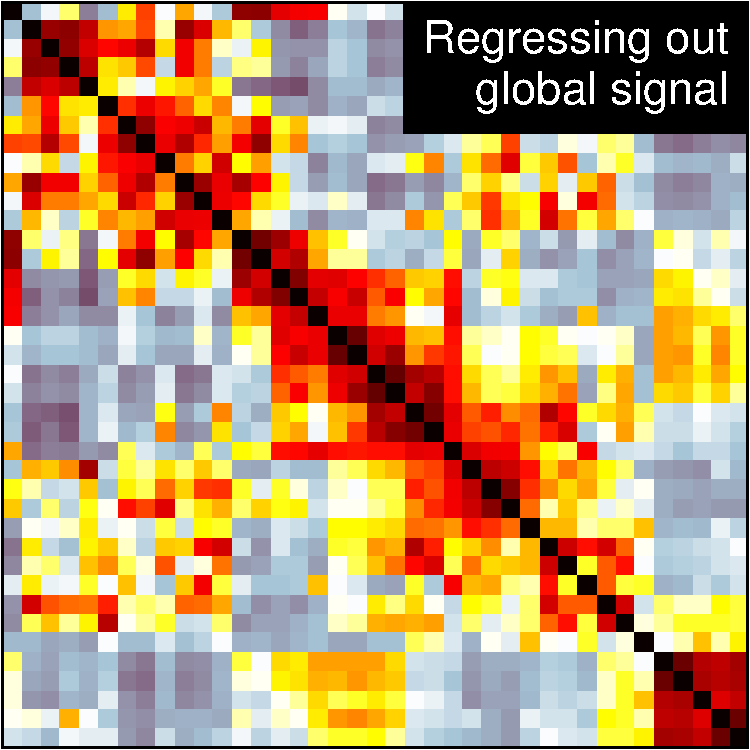
\includegraphics[width=\linewidth]{group_emp_cov_global_mean.pdf}%
\end{minipage}%

% XXX: need to give details on the dataset used here

\caption{
Correlation matrices of rest time-series extracted from the 39 main
regions of the Varoquaux 2011 \cite{varoquaux2011} parcellation with
different choices of confound regressors -- 
\textbf{Left}: regressing out CompCor signals, as well as white matter and
CSF average signals and movement parameters. The insert shows the
connections restricted to a few major nodes.
-- \textbf{Upper right}: regressing out only movement parameters. -- 
\textbf{Lower right}:
regressing out movement parameters and global signal mean.
No frequency filtering was applied here.
\label{fig:correlation_matrices}
When no confounding brain signals are regressed, all regions are heavily
correlated. Regressing out common signal, in the form of well-identified
confounds or a global mean, teases out the structure.
}
\end{figure}
%---------------------------------------------------------------------------}}}

% The following paragraph is convoluted: we start to say that rest is
% from time-series, and task from beta, we go on discussing about beta
% maps, and then we move back to rest. It might need restructuring

% Horrible sentence below

\paragraph{Signal extraction and cleaning}
Given graph nodes, the next step 
Given ROIs, the next step is to extract from them a summary measure. To
study \emph{on-going} activity, \emph{e.g.}\ with rest data, signal
extraction is performed from the EPI time series; however, to study
\emph{evoked} activity with task-driven studies it can be beneficial to
run a GLM-based first-level analysis, enforcing specificity of the measure
extracted to the task. With slow event-related designs, task-specific
functional connectivity can be captured in trial-to-trial fluctuations in
the BOLD response, estimated using a GLM analysis with one regressor per
trial \cite{grillon2012,rissman2004}. This approach, known as beta-series
regression, has been adapted for rapid event-related designs, using
multiple GLMs to optimize deconvolution of each trial \cite{mumford2012}.
With rest datasets, it is important to regress out time series capturing
movement and other sources of structured noise, to separate on-going
activity from confounding signals. In addition to removing movement
parameters estimated during preprocessing, removing linear trends, signal
extracted from the white matter and the CSF \cite{chang2009}, as well as
using the CompCor \cite{behzadi2007} procedure gives more contrasted
correlation matrices that outline functional structures better
(fig.\,\ref{fig:correlation_matrices}). 
Indeed, white matter and CSF signals capture thermal noise, 
systematic variation due to multichannel head coils, cardiac and resp.
smaller motions, physiological noise correction.
Filtering high frequencies is
often recommended, based on the initial observation that neural-related
signals are observed below 0.1\,Hz \cite{cordes2001,biswal1995}. While
high-pass and low-pass filtering decrease the impact of some confounds,
recent studies have shown that information on neural processes is present
in the full spectrum of frequencies observed
\cite{smith2012,vanoort2012}. Regressing out a good choice of confound
signals is more specific than frequency filter, and in our experience
gives more contrasted correlation matrices\footnote{Note that naive use
of filtering can induce spurious correlations \cite{davey2012}.}.

Finally, it is important to keep in mind that using resting-state to
study on-going activity is fragile to confounds such as movement
\cite{vandijk2012,power2011} or scanner noise, and probably more so than
activation studies as it is harder to control the specificity of the
signal extracted. Special care must be taken in preprocessing strategies
\cite{vandijk2010,satterthwaite2012}.
%
In addition, improved specificity to BOLD signal can be enforced by
using only signal in voxels near gray-matter tissues. For this purpose,
we suggest summarizing the signal in an ROI by a mean of the different voxels
weighted by the subject-specific gray matter probabilistic segmentation,
% CAMERON why only SPM's tool?
% GAEL: afaik, it only gives hard segmentation, and not probabilistic
% segmentation
as output by \emph{e.g.}\ SPM's segmentation tool \cite{ashburner2005}.

% CAMERON TODO: two sentences max
% Regressing out task?? Skipping for lack of space


%{{{------ Precision matrices figure -----------------------------------------
\begin{figure}
\newcommand{\photoframe}[1]{\setlength\fboxsep{0pt}%
{\color{black!70}\fbox{#1}\color{black}}}%
\begin{minipage}{.666\linewidth}%
    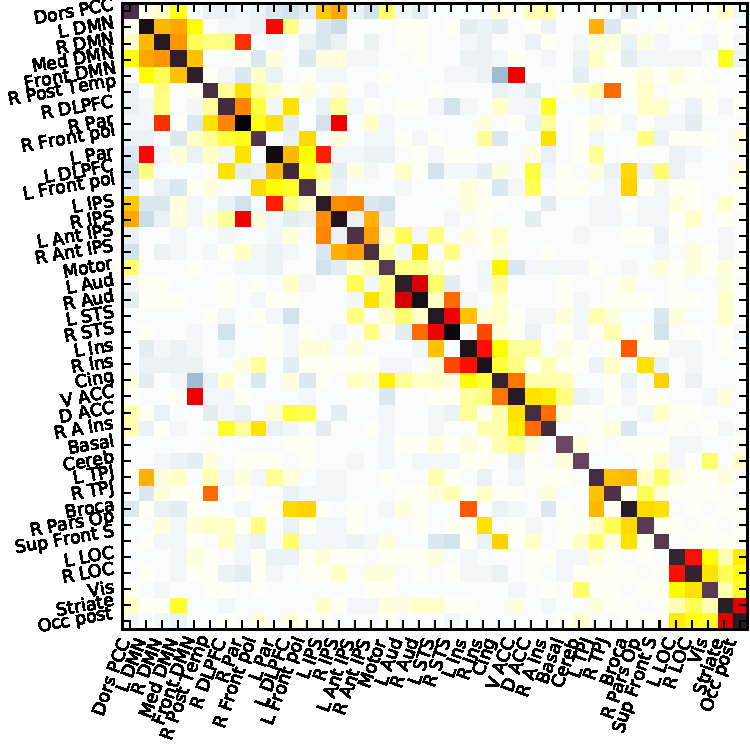
\includegraphics[width=\linewidth]{group_l21_prec.pdf}%
    \raisebox{.606\linewidth}{%
	\hspace*{-.462\linewidth}%
	\photoframe{%
	%\setlength\fboxsep{1pt}%
	\colorbox{white}{%
	\raisebox{.003\linewidth}{%
	    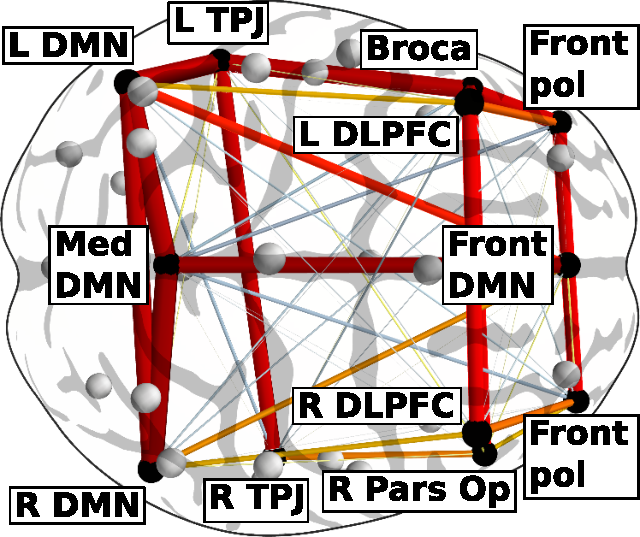
\includegraphics[width=.455\linewidth]{group_l21_prec_3d_labels}}%
	\rule{0pt}{.387\linewidth}%
	}}%
    }
\end{minipage}%
\hspace*{1pt}%
\begin{minipage}{.33\linewidth}%
    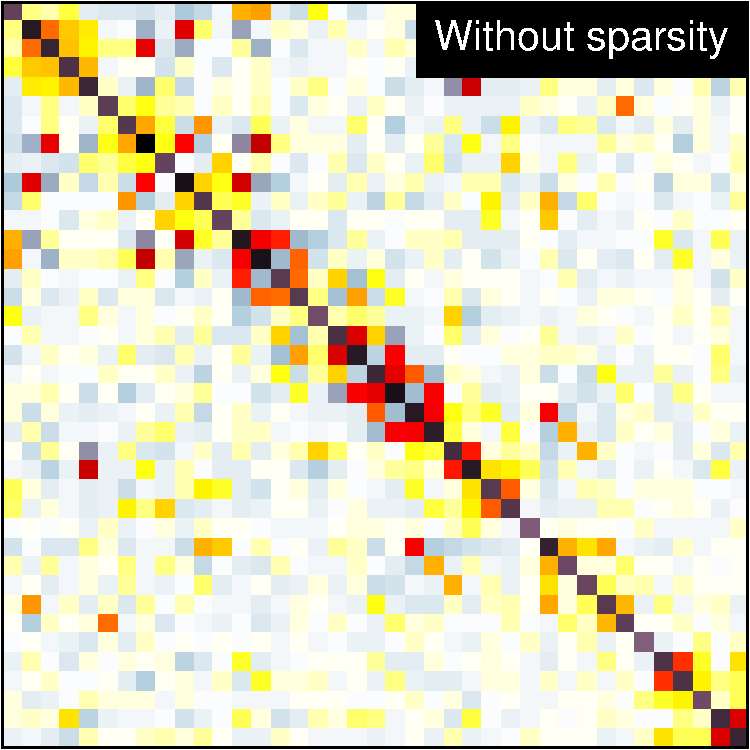
\includegraphics[width=\linewidth]{group_emp_prec.pdf}%

    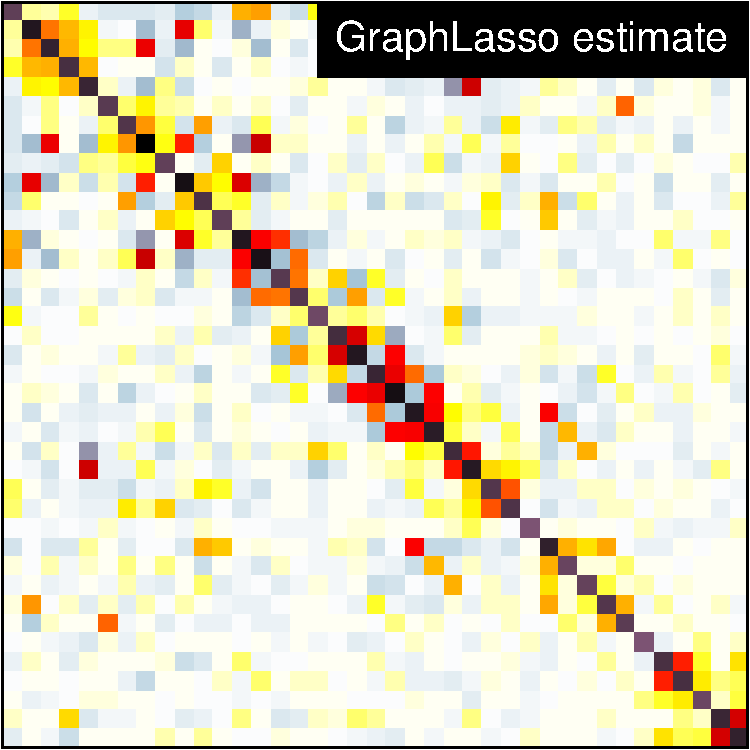
\includegraphics[width=\linewidth]{group_l1_prec.pdf}%
\end{minipage}%

\caption{
Different inverse-covariance matrices estimates corresponding to
fig.\,\ref{fig:correlation_matrices} -- \textbf{Left}: group-sparse estimate
using the $\ell_{21}$ estimator \cite{varoquaux2010c}.
The insert shows the
connections restricted to a few major nodes. -- \textbf{Upper
right}: non-sparse estimate: inverse of the sample correlation matrix. --
\textbf{Lower right}: sparse estimate using the Graph Lasso
\cite{friedman2008}.
\label{fig:icov_estimators}
}
\end{figure}
%---------------------------------------------------------------------------}}}


\paragraph{Correlation and partial correlations}
%
Given ROIs defining nodes the nodes of the functional-connectome graph,
one need to estimate the corresponding edges connecting them.
Functional connectivity between the ROIs can be measured by computing the
correlation matrix of the extracted signals. An important and often
neglected point is that the sample correlation matrix, \emph{i.e.}\ the
correlation matrix obtained by plugging the observed signal in the
correlation matrix formula, is not the population correlation matrix,
\emph{i.e.}\ the correlation matrix of the data-generating process. If the
% CAMERON THIS IS ALSO DETERMINED BY TEMPORAL AUTOCORRELATIONS! band-limited
% by hemodynamic response, low sampling frequency
number of measurements was infinite, the two would coincide, however if
this number is not large compared to the number of connections (that
scales as the square of the number of ROIs), the sample correlation
matrix is a poor estimate of the underlying population correlation
matrix. In other words, the sample correlation matrix captures a lot of
sampling noise, intrinsic randomness that arises in the estimation of
correlations from short time series. Conclusions drawn from the sample
correlation matrix can easily reflect this estimation error.
%
Varoquaux \emph{et al.}~\cite{varoquaux2010c} and Smith \emph{et
al.}~\cite{smith2011} have shown respectively on rest fMRI and on
realistic simulations that a good choice of correlation matrix estimator
could recover the connectivity structure, where the sample correlation
matrix would fail.  In general, the choice of a better estimate depends on
the settings and the end goals \cite{varoquaux2012,varoquaux2010b},
however the Ledoit-Wolf shrinkage estimate \cite{ledoit2004} is a simple,
computationally-efficient, and parameter-less alternative that performs
uniformly better than the sample correlation matrix
\cite{varoquaux2012,varoquaux2010c} and should always be preferred.


%{{{------ Regressor in precision matrix -------------------------------------
\begin{figure}
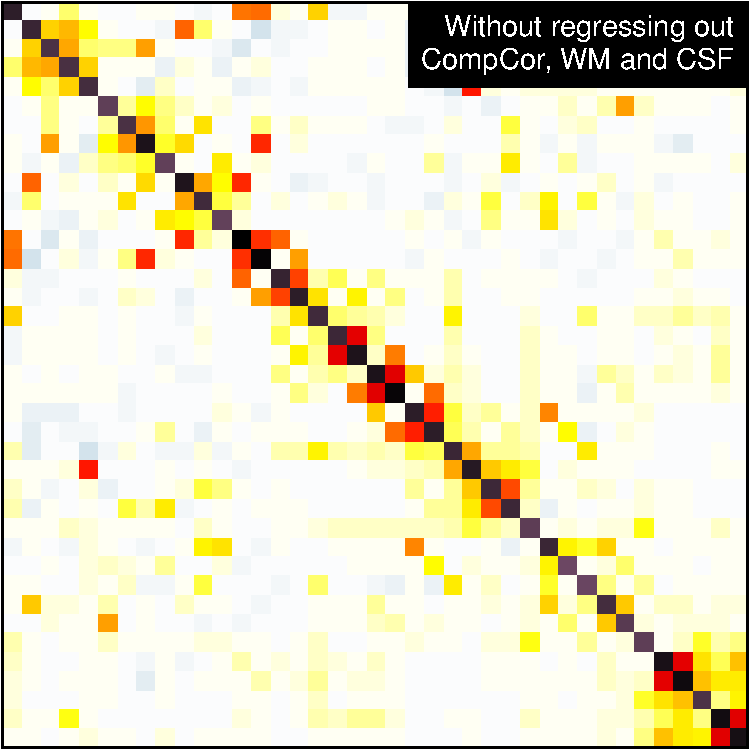
\includegraphics[height=.482\linewidth]{group_l21_prec_no_confounds.pdf}%
\hspace*{1pt}%
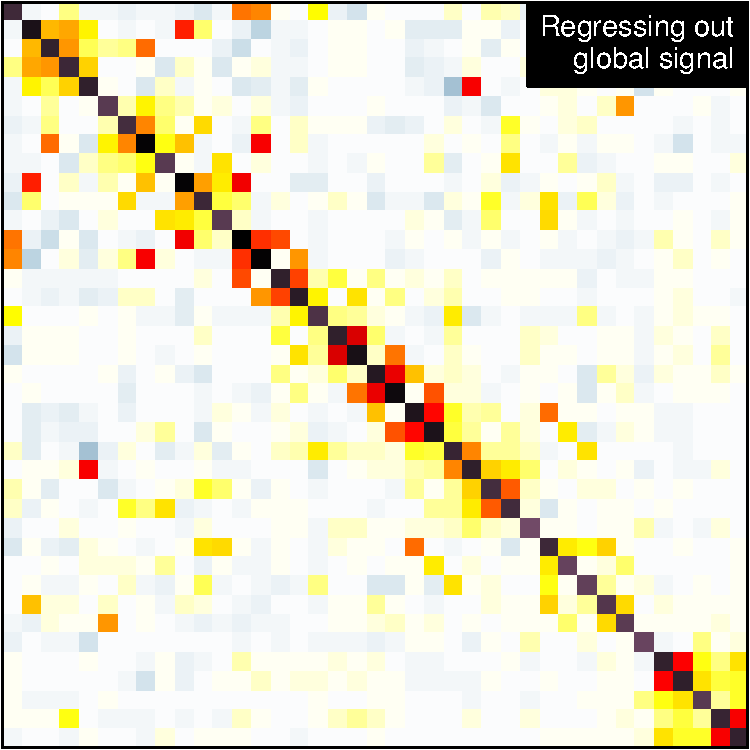
\includegraphics[height=.482\linewidth]{group_l21_prec_global_mean.pdf}%
\hspace*{1pt}%

\includegraphics[height=.482\linewidth]{cmap.pdf}%

\caption{Inverse covariance matrices for different choice of
confound regressors --
\label{fig:icov_regressors}
\textbf{Left}: regressing out only movement parameters --
\textbf{Right}: removal of the global mean,
instead of the white matter, CSF, and CompCor time courses. 
}
\end{figure}
%---------------------------------------------------------------------------}}}



For the problem of recovering the functional-connectivity
\emph{structure}, \emph{i.e.}\ finding which region is connected to
which, sparse inverse covariance estimators have been found to be
% CAMERON Isn't there a paper from Stanford about this as well??
efficient \cite{varoquaux2010c, smith2011}. The intuition for relying on
inverse covariance rather than correlation stems from that fact that
standard correlation (marginal correlation) between two variables $a$ and
$b$ also capture the effects of other variables: strong correlation of
$a$ and $b$ with a third variable $c$ will induce a correlation between
$a$ and $b$. On the opposite, the inverse covariance\footnote{Covariance
and correlation matrices differ simply by the fact that a covariance
matrix captures the amplitude of a signal, via its variance, while a
correlation matrix is computed on standardized (zero mean, unit variance) signals.}
matrix captures
partial correlations, removing the effect of other variables
\cite{marrelec2006a}. In the small sample limit, this removal is
challenging from the statistical standpoint, and an assumption of sparsity,
\emph{i.e.}\ that only few variables need to be considered at a time, is
important to estimate a good inverse covariance. Various estimation
strategies exist for sparse inverse covariance, and have an impact on the
resulting networks \cite{varoquaux2012,varoquaux2010c}. The
Graph Lasso ($\ell_1$-penalized maximum-likelihood estimator)
\cite{friedman2008} is in general a good approach for structure recovery. In group studies,
the $\ell_{21}$ estimator \cite{varoquaux2010c,honorio2012} is useful to
impose a common sparsity structure across different subjects and achieve
better recovery of this common structure. Simply put, these approaches
are necessary because estimation noise creates a background structure
(see fig.\,\ref{fig:icov_estimators}); however, unlike in a univariate situation, the
parameters are not independent, and the spurious background connections
degrade the estimation of the actual connections. The sparse estimators
make a compromise between imposing simpler models, \emph{i.e.}\ with less
% CAMERON "fitting well the data" needs to be fixed
connections, and fitting well the data. This compromise is set via a
regularization parameter which controls the sparsity of the estimate. A
good rule of thumb to choose this parameter is via cross-validation
\cite{varoquaux2010c}.

% CAMERON should you discuss limitations to the L1 norm, such as bounding
% the number of non-zero weights by the number of observations: does this
% only apply to regressions?

% XXX: must comment on the estimator figure

\paragraph{Network structure extracted}
%
The correlation matrices and inverse-covariance matrices that we extract
contain a lot of information on the functional structure of the brain.
First, the correlation matrix (fig.\,\ref{fig:correlation_matrices})
shows blocks of coactivating regions that can be interpreted as
large-scale functional networks, such as the default mode network. Note
% CAMERON How about spectral reordering?
that the split in networks is not straightforward. Different ordering of the
nodes will reveal different networks. 
% CAMERON I don't get this sentence
Indeed, because of the presence of
hubs and interleaved networks, the picture in terms of segregated networks
is not sufficient to explain full-brain connectivity
\cite{varoquaux2012}. Connectivity matrices, correlation matrices and
inverse-covariance matrices, can be represented as graphs: nodes connected
by weighted edges (inserts on fig.\,\ref{fig:correlation_matrices} and
fig.\,\ref{fig:icov_estimators}). The inverse-covariance matrix, which
captures partial correlations, appears then as extracting a
\emph{backbone} or \emph{core} of the graph.
% CAMERON This is a really long sentence
While such structure has
been used as a way to summarize anatomical brain connectivity graphs
\cite{hagmann2008}, here it has a clear-cut meaning with regards to
% CAMERON BOLD not explicitly defined
the BOLD signal: it gives the conditional independence structure between
regions \cite{varoquaux2012}. In other words, regions $a$ and $b$ are
not connected if the signal that they have in common can be explained by
a third region $c$. In this light, the choice of nuisance regressors to
remove confounding common signal is less critical with partial
correlations than with correlations. Indeed, while with
correlation matrices regressing out the global mean has a drastic effect
(fig.\,\ref{fig:correlation_matrices} upper right and lower right), on
inverse covariance it only changes very slightly the resulting matrices
(fig.\,\ref{fig:icov_regressors}). 
% CAMERON I would move this to preprocessing section
There have been debates on whether to
regress out certain signals, such as the global mean,  as it induces
negative correlations \cite{murphy2009,chang2009,fox2009}, and these may seem
% CAMERON "doing the opposite of the other" is a bit odd
surprising: one network is doing the opposite of the other. However,
correlation between two signals only takes its meaning with the
definition of a baseline. A simple picture to explain anti-correlations
between two regions is the presence of a third region, mediating the
interactions. Using this third region as a baseline would amount to
estimate partial correlations in the whole system. Using 
inverse-covariance matrices or partial correlations to understand brain
connectivity makes the interpretation in terms of interactions between
brain regions easier and more robust to the choice of confounds.

% XXX: where to insert this in the above paragraph: cite the
% Fransson/Marrelec paper on the role of the PCC

% \cite{chai2011} (note: chai2011 used compcor)
% Remark that partial correlations consistently have no negative values.


%%%%%%%%%%%%%%%%%%%%%%%%%%%%%%%%%%%%%%%%%%%%%%%%%%%%%%%%%%%%%%%%%%%%%%%%%%%%%%%

\section{Comparing connectivity}

We now turn to the problem of comparing functional
connectivity across subjects or across conditions.

%------------------------------------------------------------------------------
\subsection{Detecting changing connections}

First, we focus on detecting where the connectivity matrices estimated in
the previous section differ.

\paragraph{Mass-univariate approaches}
%
% CAMERON there has to be other references ...
The most natural approach is to apply a linear model to each coefficient of
the connectivity matrices \cite{lewis2009,grillon2012}. This
approach is similar to the second-level analysis used in mass-univariate
brain mapping, and gives rise to many of the well-known techniques
used in such a context, such as the definition of a second-level design,
with possibly the inclusion of confounding effects, and statistical tests
(T tests or F tests) on contrast vector. Importantly, in order to work
with Gaussian-distributed variables, it is necessary to apply a Fisher
Z transform\footnote{See
\url{http://en.wikipedia.org/wiki/Fisher_transformation} or
\cite{anderson1958} section 4.2.3 for mathematical arguments.} to the
correlations. Note that
in these settings, the Ledoit-Wolf estimator \cite{ledoit2004} is
often a good choice to estimate the correlation matrix, as it is
parameter-free and gives good estimation performance without imposing any
restrictions on the data.
%
For hypothesis testing,
correcting for multiple comparison can severely limit statistical
power, as the number of tests performed scales as the square of the
number of regions used. Controlling for the false discovery rate (FDR)
mitigates this problem. Alternatively, as the assumptions underlying the
Benjamini-Hochberg procedure \cite{benjamini1995} for the FDR can easily
be broken, non-parametric permutations-based tests give reliable
approaches. In particular, the max-T procedure \cite{ge2003,nichols2001}
is interesting to avoid the drastic Bonferroni correction when
controlling for multiple comparison in family-wise error rate.

% CAMERON what about CWAS or Bellec??

%{{{------ Inter subject fluctuations ----------------------------------------
\begin{figure}
\hspace*{.5ex}%
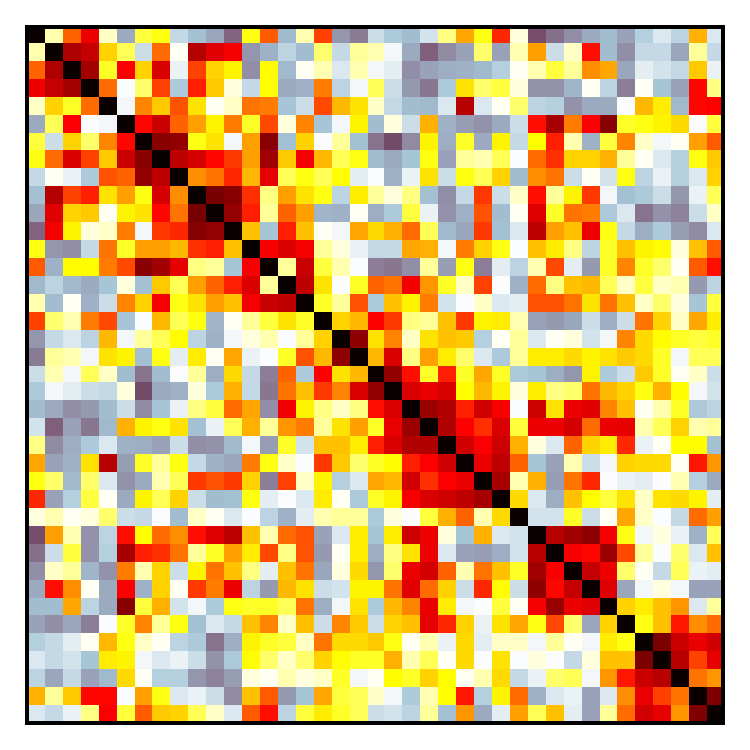
\includegraphics[width=.196\linewidth]{inter_subj/cov_sub00.pdf}%
\hspace*{-.2ex}%
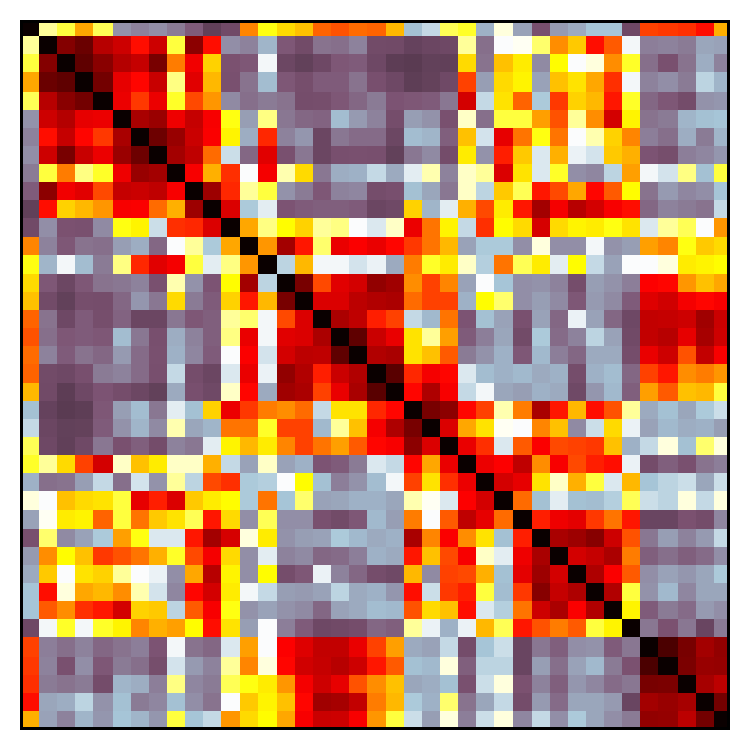
\includegraphics[width=.196\linewidth]{inter_subj/cov_sub29.pdf}%
\hspace*{-.2ex}%
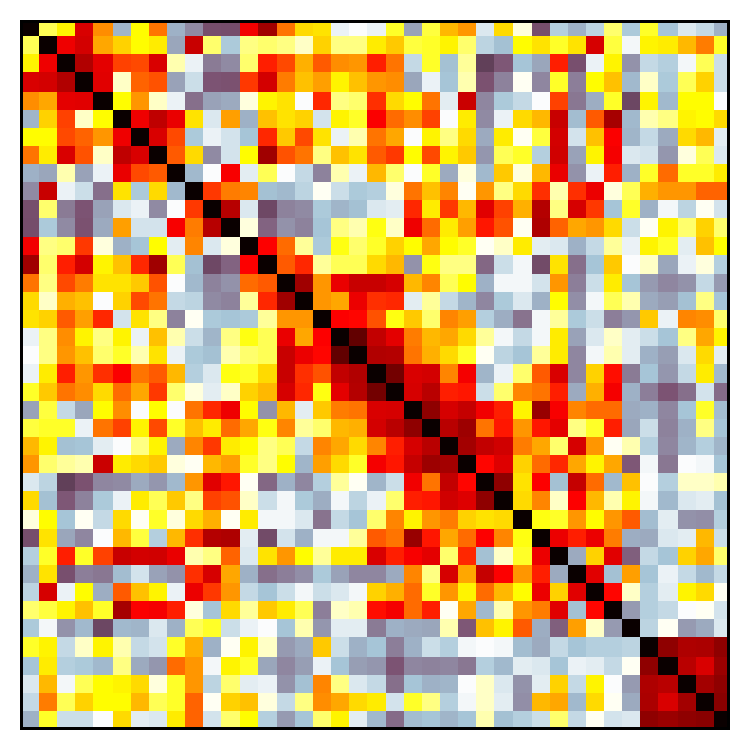
\includegraphics[width=.196\linewidth]{inter_subj/cov_sub01.pdf}%
\hspace*{-.2ex}%
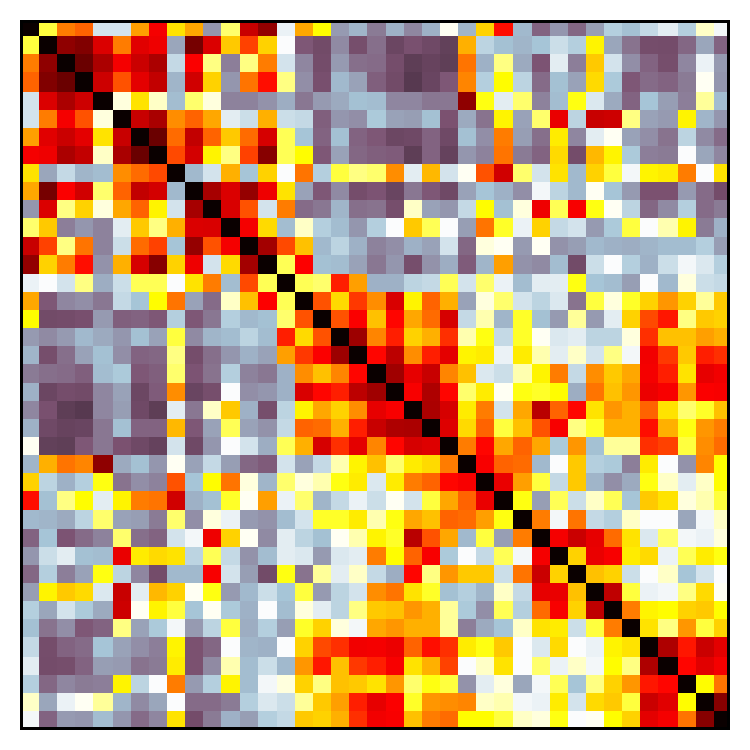
\includegraphics[width=.196\linewidth]{inter_subj/cov_sub07.pdf}%
\hspace*{-.2ex}%
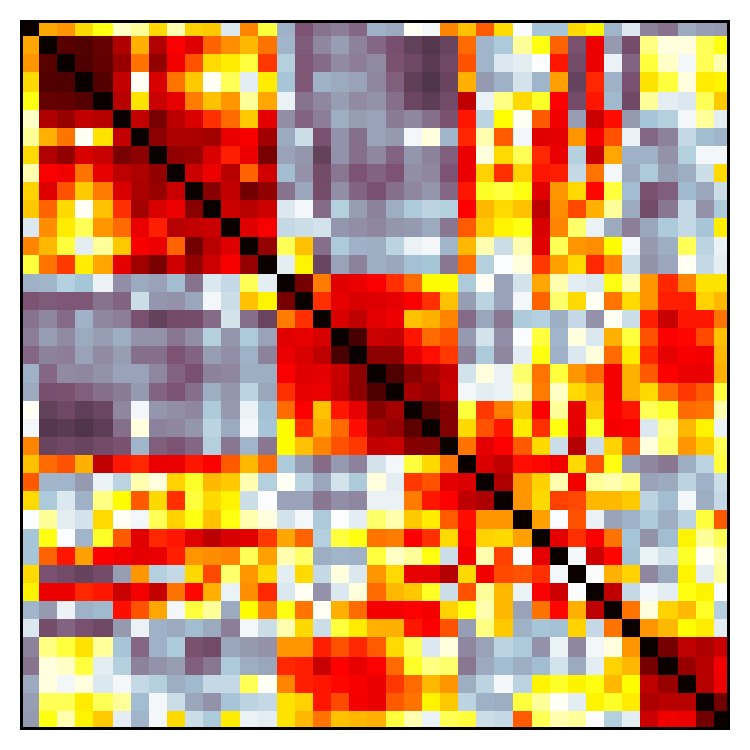
\includegraphics[width=.196\linewidth]{inter_subj/cov_sub53.pdf}%
\hspace*{.1ex}%
\raisebox{.005\linewidth}{%
    
\includegraphics[width=.0186\linewidth]{cmap_00.pdf}%
    \llap{
	\raisebox{.003\linewidth}{%
	    \bfseries\tiny\color{white} -\!1\hspace*{-.2ex}}%
    }%
    \llap{
	\raisebox{.17\linewidth}{%
	    \bfseries\tiny\color{white} 1\hspace*{.1ex}}%
    }%
}%
\llap{\rlap{
    \setlength\fboxsep{1pt}%
    \raisebox{.16\linewidth}{%
	\colorbox{black!10}{%
	    \sffamily\small\textbf{a}. Correlation matrices}}%
	}%
    \hspace*{.993\linewidth}%
}


\hspace*{.5ex}%
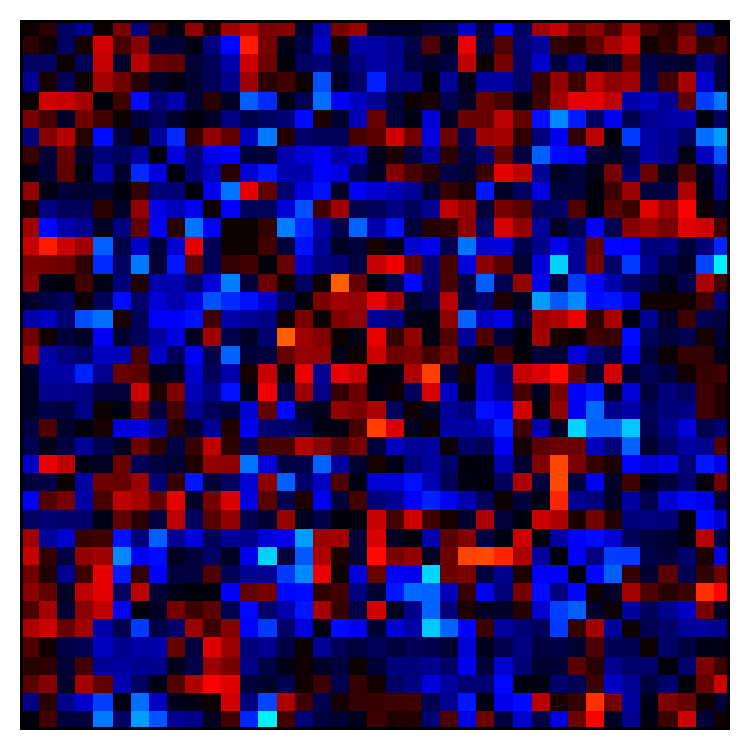
\includegraphics[width=.196\linewidth]{inter_subj/z_score_sub00.pdf}%
\hspace*{-.2ex}%
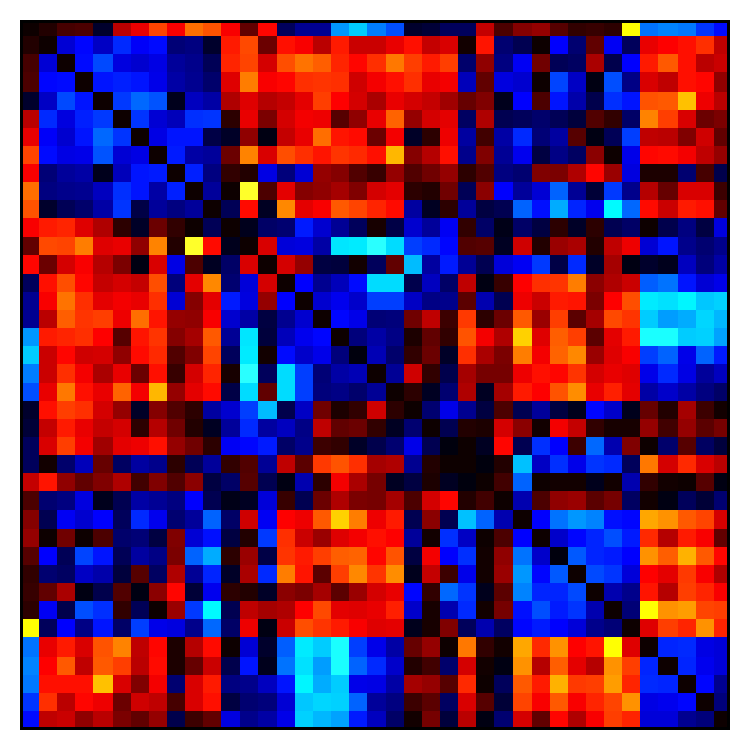
\includegraphics[width=.196\linewidth]{inter_subj/z_score_sub29.pdf}%
\hspace*{-.2ex}%
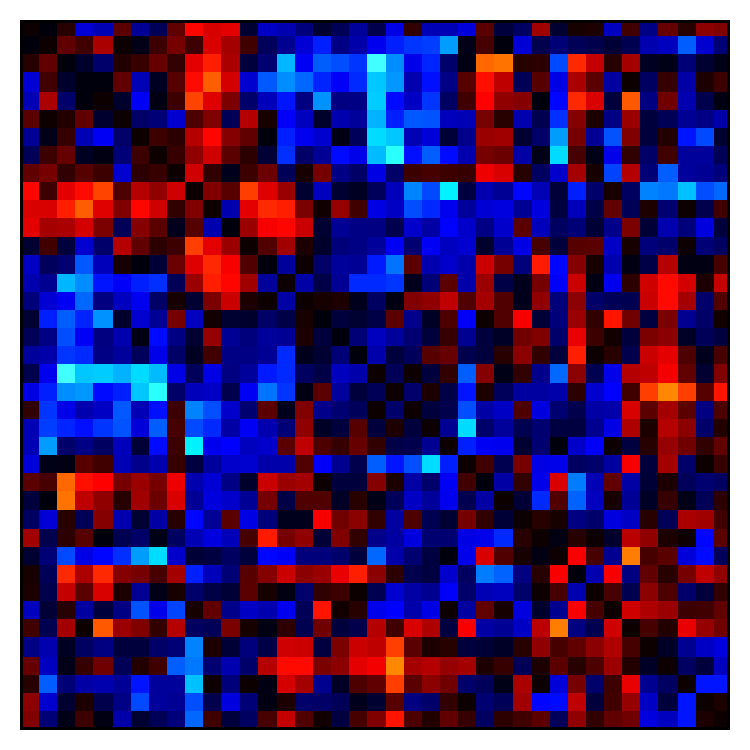
\includegraphics[width=.196\linewidth]{inter_subj/z_score_sub01.pdf}%
\hspace*{-.2ex}%
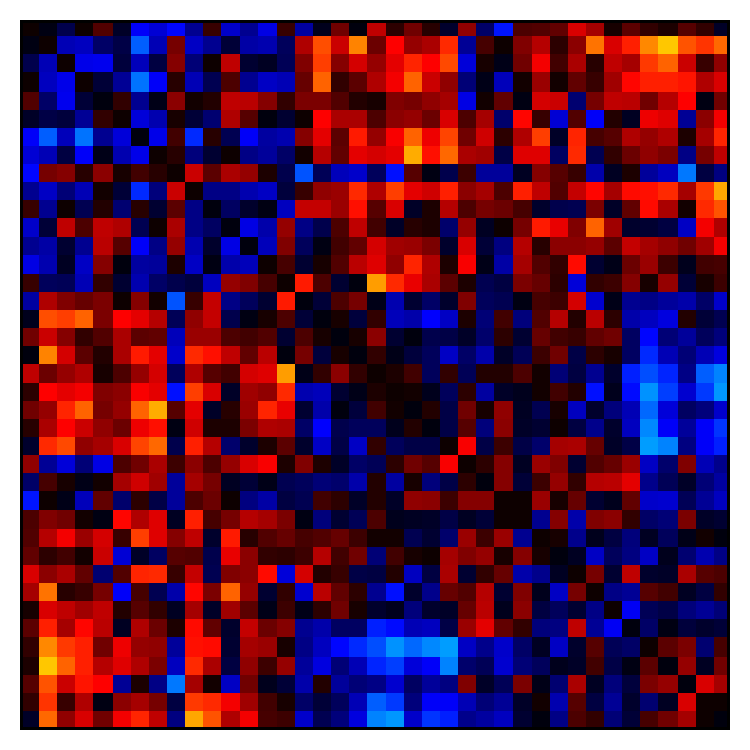
\includegraphics[width=.196\linewidth]{inter_subj/z_score_sub07.pdf}%
\hspace*{-.2ex}%
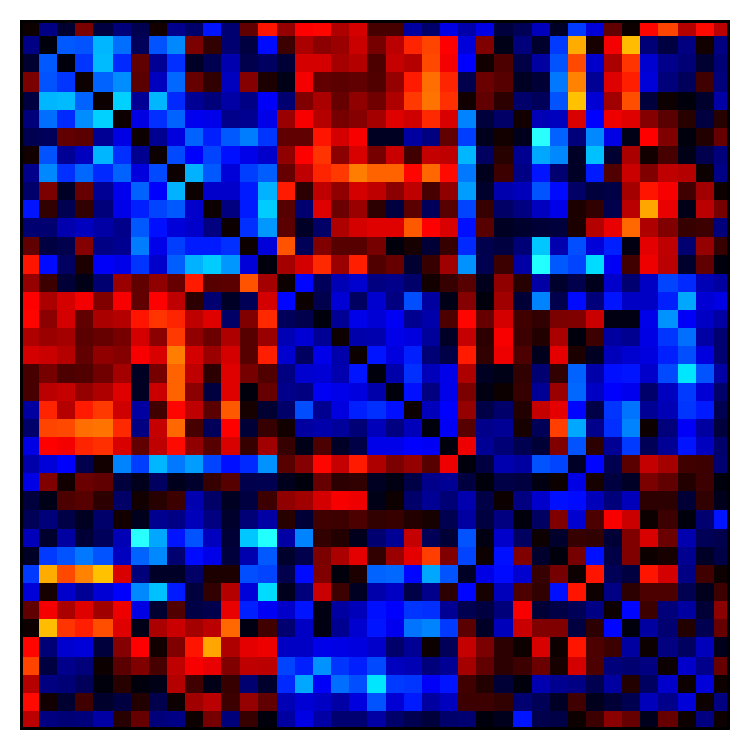
\includegraphics[width=.196\linewidth]{inter_subj/z_score_sub53.pdf}%
\hspace*{.1ex}%
\raisebox{.005\linewidth}{%
    
\includegraphics[width=.0186\linewidth]{cmap_01.pdf}%
    \llap{
	\raisebox{.003\linewidth}{%
	    \bfseries\tiny -\!\hspace*{-.1ex}4\hspace*{-.1ex}}%
    }%
    \llap{
	\raisebox{.168\linewidth}{%
	    \bfseries\tiny 4\hspace*{.1ex}}%
    }%
}%
\llap{\rlap{
    \setlength\fboxsep{1pt}%
    \raisebox{.16\linewidth}{%
	\colorbox{black!10}{%
	    \sffamily\small\textbf{b}. Z score on difference}}%
	}%
    \hspace*{.993\linewidth}%
}

\hspace*{.5ex}%
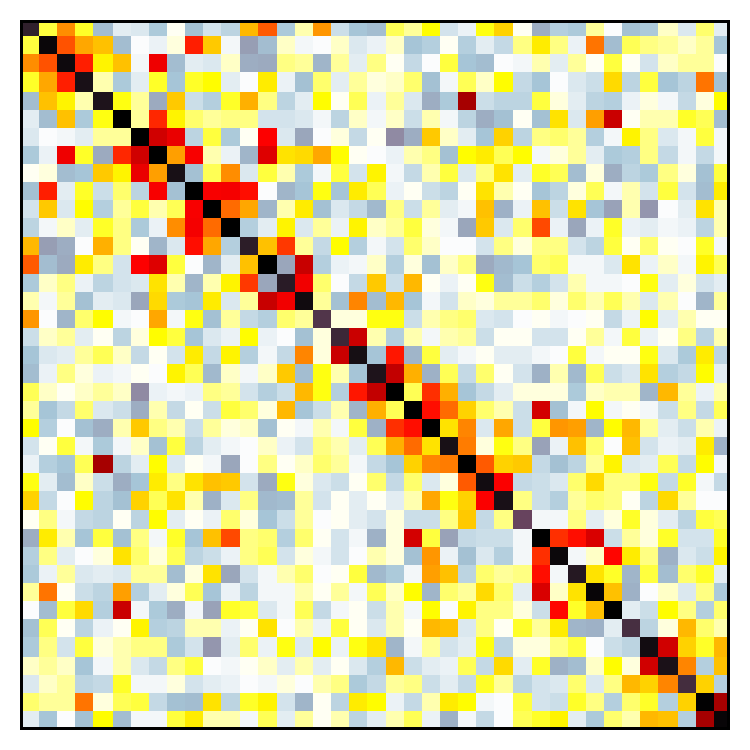
\includegraphics[width=.196\linewidth]{inter_subj/prec_sub00.pdf}%
\hspace*{-.2ex}%
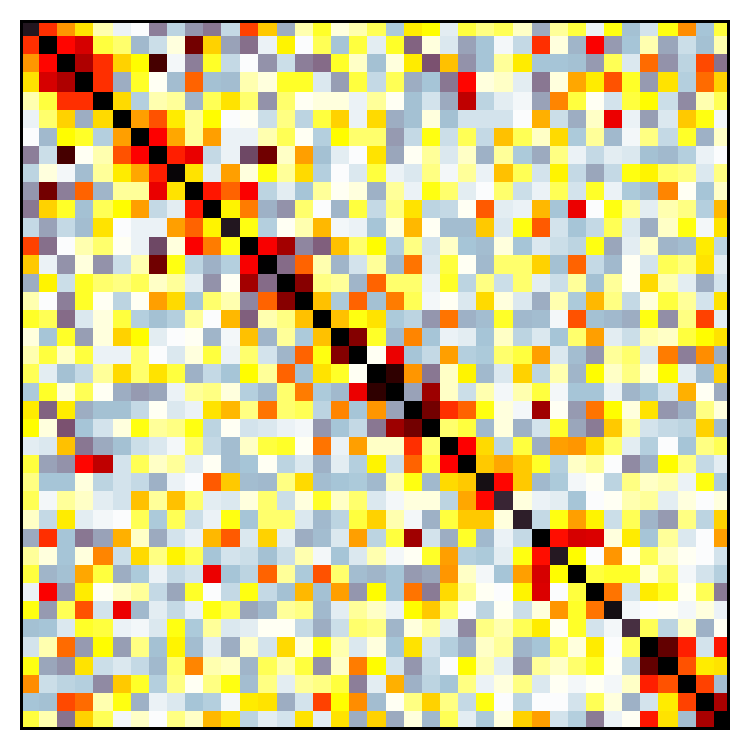
\includegraphics[width=.196\linewidth]{inter_subj/prec_sub29.pdf}%
\hspace*{-.2ex}%
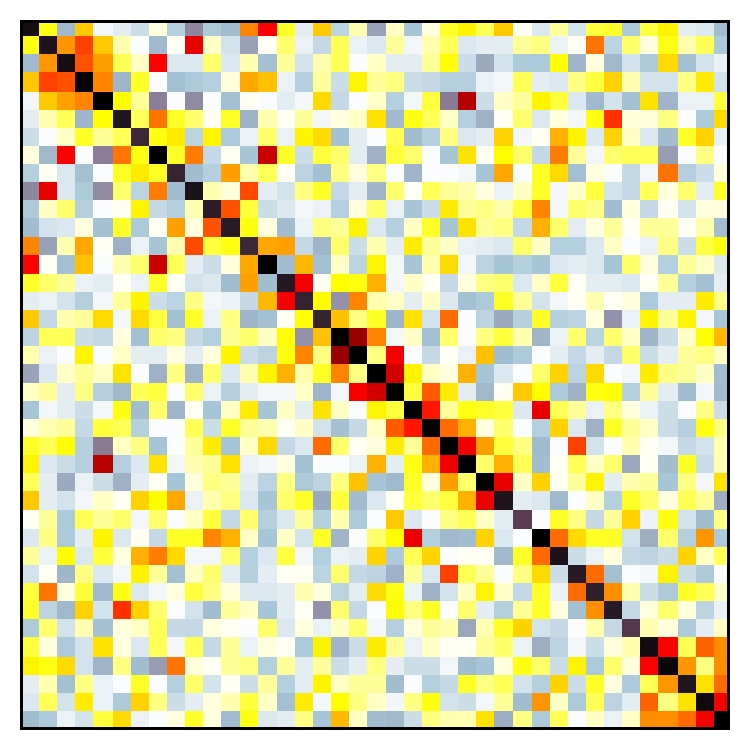
\includegraphics[width=.196\linewidth]{inter_subj/prec_sub01.pdf}%
\hspace*{-.2ex}%
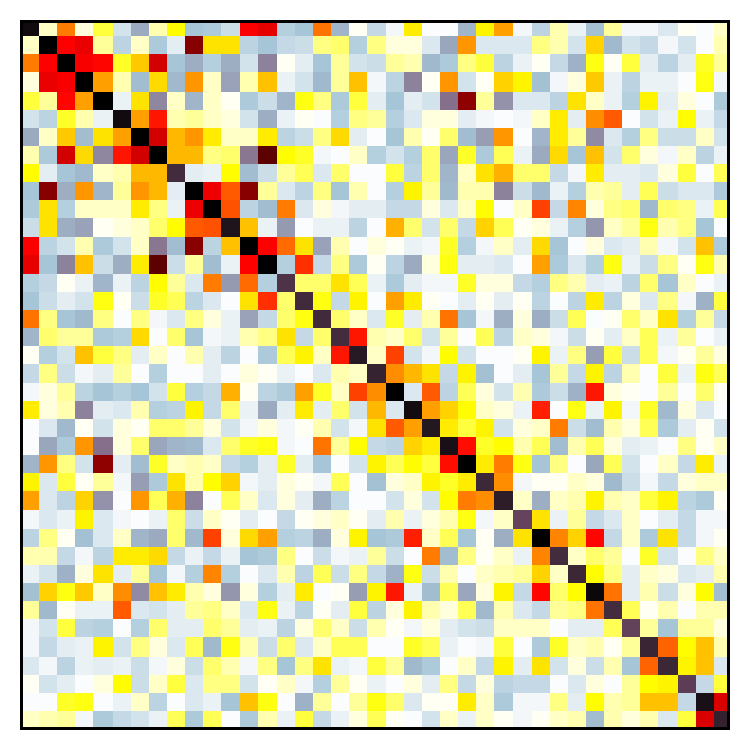
\includegraphics[width=.196\linewidth]{inter_subj/prec_sub07.pdf}%
\hspace*{-.2ex}%
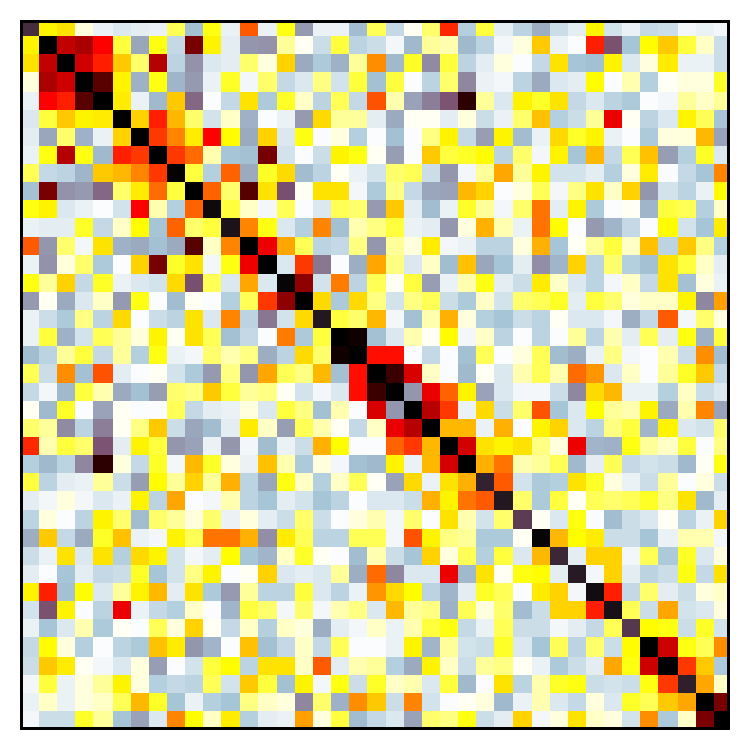
\includegraphics[width=.196\linewidth]{inter_subj/prec_sub53.pdf}%
\hspace*{.1ex}%
\raisebox{.005\linewidth}{%
    
\includegraphics[width=.0186\linewidth]{cmap_00.pdf}%
    \llap{
	\raisebox{.003\linewidth}{%
	    \bfseries\tiny\color{white} -\!1\hspace*{-.2ex}}%
    }%
    \llap{
	\raisebox{.17\linewidth}{%
	    \bfseries\tiny\color{white} 1\hspace*{.1ex}}%
    }%
}%
\llap{\rlap{
    \setlength\fboxsep{1pt}%
    \raisebox{.16\linewidth}{%
	\colorbox{black!10}{%
	    \sffamily\small\textbf{c}. Inverse-covariance matrices}}%
	}%
    \hspace*{.993\linewidth}%
}

\hspace*{.5ex}%
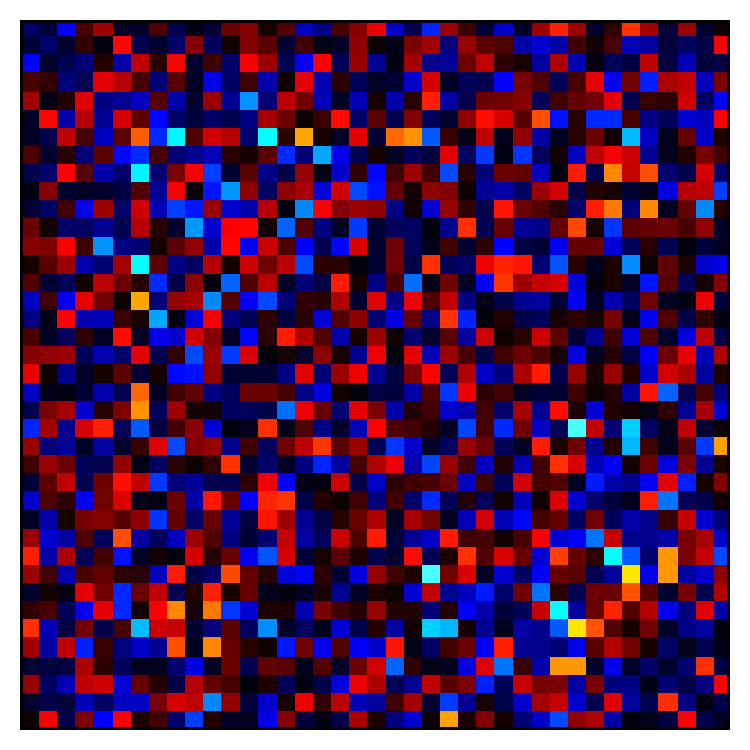
\includegraphics[width=.196\linewidth]{inter_subj/z_score_prec_sub00.pdf}%
\hspace*{-.2ex}%
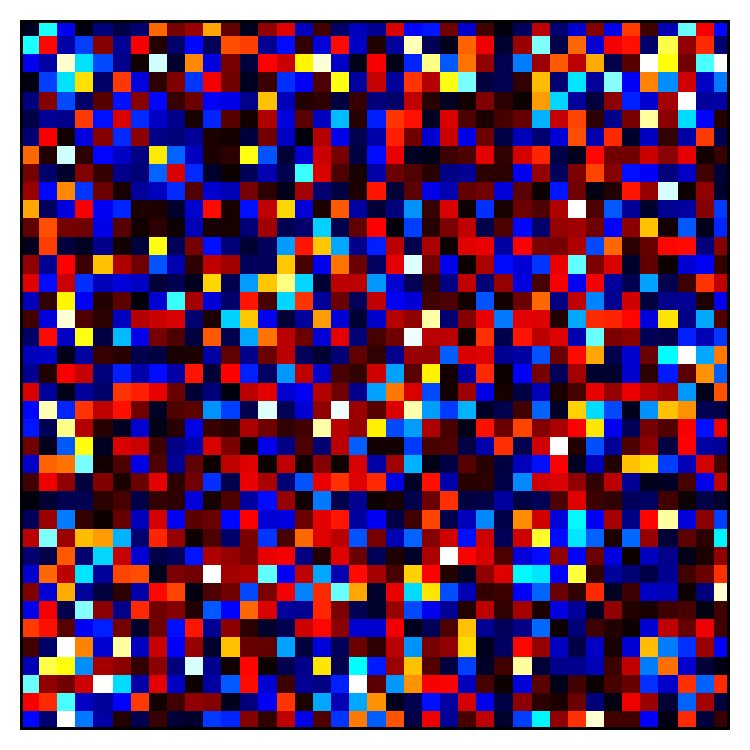
\includegraphics[width=.196\linewidth]{inter_subj/z_score_prec_sub29.pdf}%
\hspace*{-.2ex}%
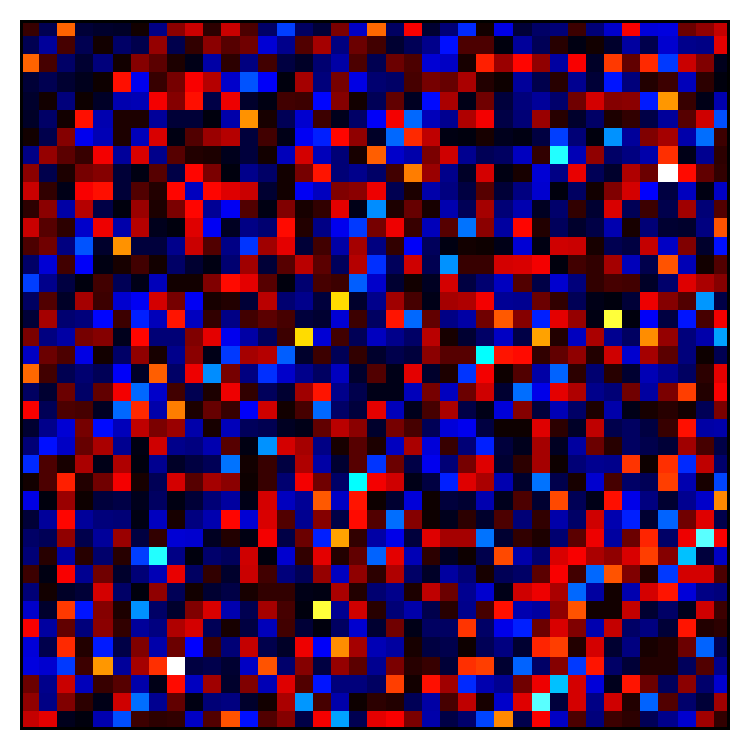
\includegraphics[width=.196\linewidth]{inter_subj/z_score_prec_sub01.pdf}%
\hspace*{-.2ex}%
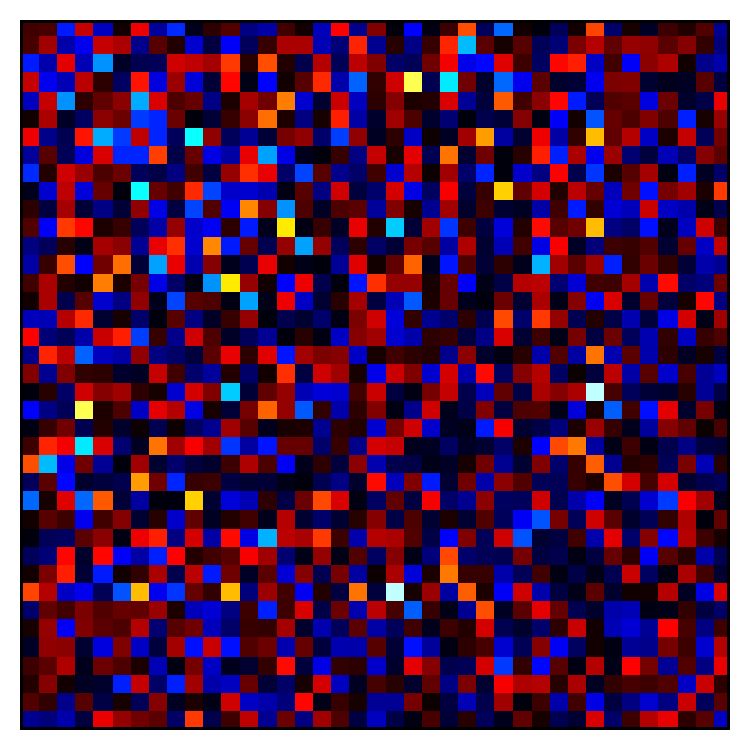
\includegraphics[width=.196\linewidth]{inter_subj/z_score_prec_sub07.pdf}%
\hspace*{-.2ex}%
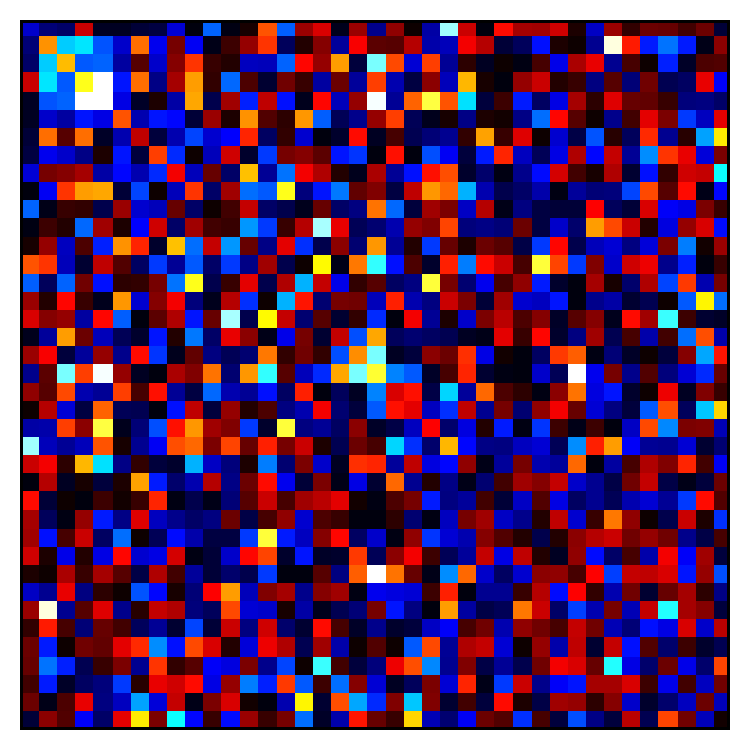
\includegraphics[width=.196\linewidth]{inter_subj/z_score_prec_sub53.pdf}%
\hspace*{.1ex}%
\raisebox{.005\linewidth}{%
    
\includegraphics[width=.0186\linewidth]{cmap_01.pdf}%
    \llap{
	\raisebox{.003\linewidth}{%
	    \bfseries\tiny -\!\hspace*{-.1ex}4\hspace*{-.1ex}}%
    }%
    \llap{
	\raisebox{.168\linewidth}{%
	    \bfseries\tiny 4\hspace*{.1ex}}%
    }%
}%
\llap{\rlap{
    \setlength\fboxsep{1pt}%
    \raisebox{.16\linewidth}{%
	\colorbox{black!10}{%
	    \sffamily\small\textbf{d}. Z score on inverse-covariance}}%
	}%
    \hspace*{.993\linewidth}%
}



\hspace*{.5ex}%
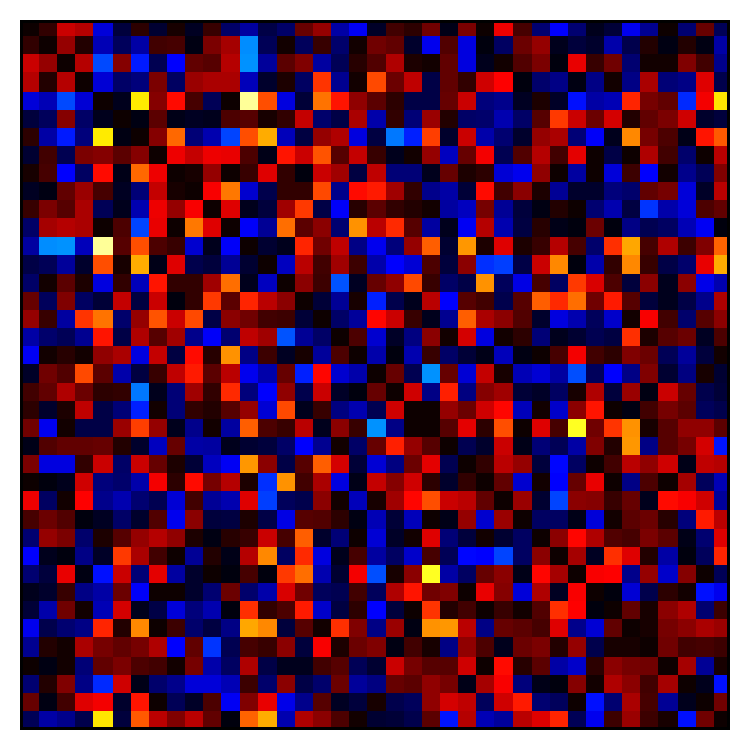
\includegraphics[width=.196\linewidth]{inter_subj/res_sub00.pdf}%
\hspace*{-.2ex}%
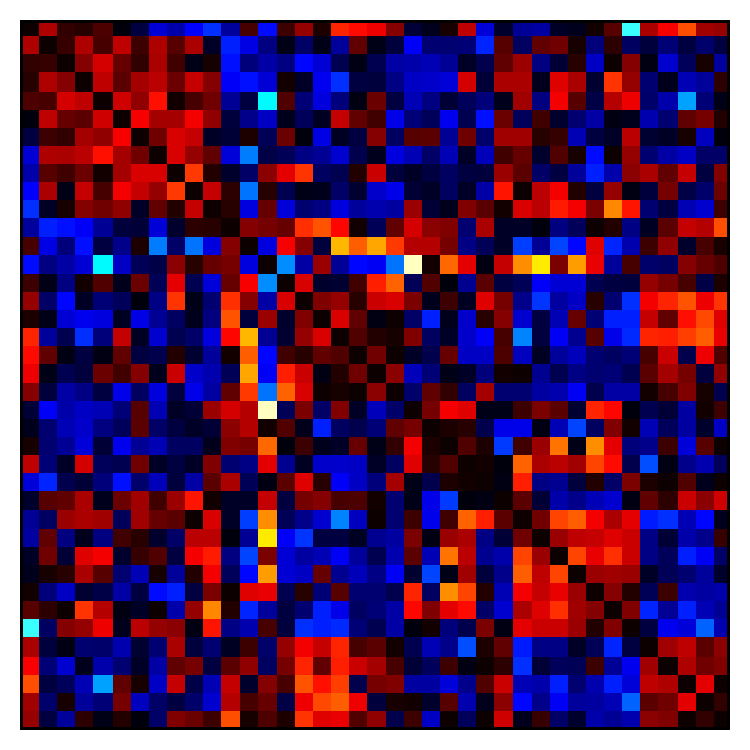
\includegraphics[width=.196\linewidth]{inter_subj/res_sub29.pdf}%
\hspace*{-.2ex}%
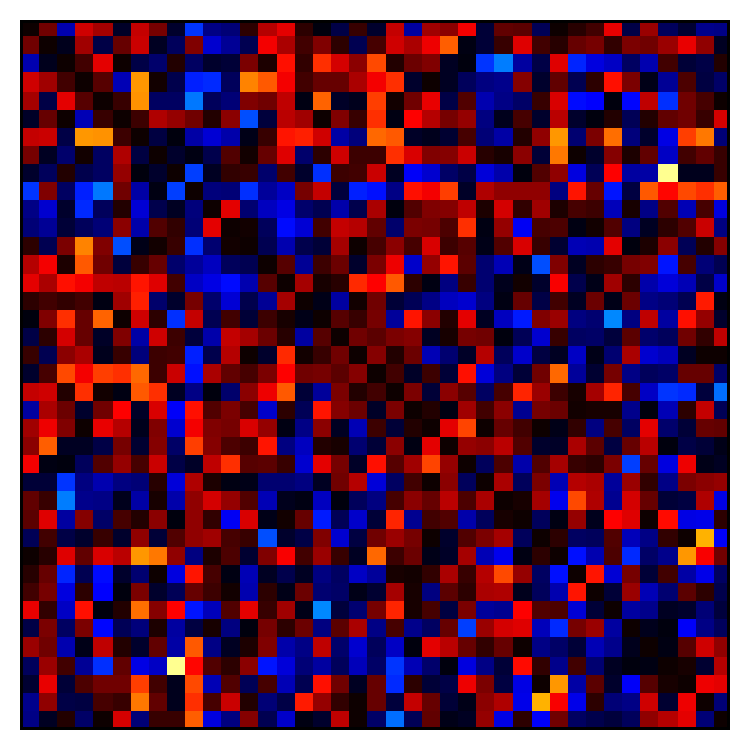
\includegraphics[width=.196\linewidth]{inter_subj/res_sub01.pdf}%
\hspace*{-.2ex}%
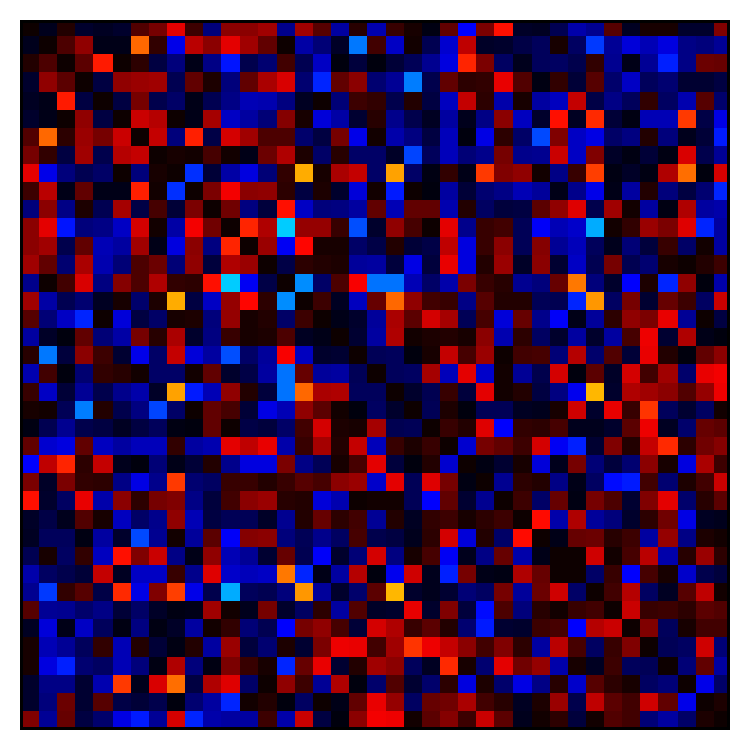
\includegraphics[width=.196\linewidth]{inter_subj/res_sub07.pdf}%
\hspace*{-.2ex}%
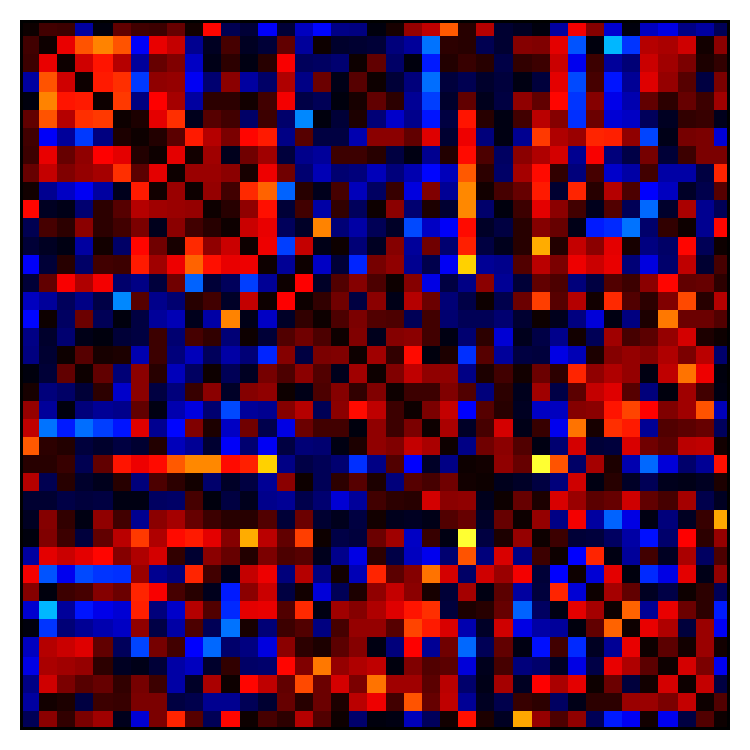
\includegraphics[width=.196\linewidth]{inter_subj/res_sub53.pdf}%
\hspace*{.1ex}%
\raisebox{.005\linewidth}{%
    
\includegraphics[width=.0186\linewidth]{cmap_01.pdf}%
    \llap{
	\raisebox{.003\linewidth}{%
	    \bfseries\tiny -\!\hspace*{-.1ex}4\hspace*{-.1ex}}%
    }%
    \llap{
	\raisebox{.168\linewidth}{%
	    \bfseries\tiny 4\hspace*{.1ex}}%
    }%
}%
\llap{\rlap{
    \setlength\fboxsep{1pt}%
    \raisebox{.16\linewidth}{%
	\colorbox{black!10}{%
	    \sffamily\small\textbf{e}. Z score on residuals \scriptsize
		\raisebox{.2ex}{\cite{varoquaux2010b}}}}%
	}%
    \hspace*{.993\linewidth}%
}

\caption{Inter subject variability. Note that this is variability
occurring in a healthy population at rest, in other words it is non specific
variability -- \textbf{a}: single-subject
correlation matrices for different subjects -- \textbf{b}:
Corresponding Z-score (effect / standard deviation) of the difference
between a subject and the remaining others -- \textbf{c}:
single-subject precision matrices -- \textbf{d}: Corresponding Z-score
for the precision matrices -- \textbf{e}:
Corresponding Z-score for the subject residuals, as defined in 
\cite{varoquaux2010b}.
\label{fig:inter_subject}}
\end{figure}
%---------------------------------------------------------------------------}}}

\paragraph{Accounting for distributed variability}
%
A specific challenge of connectivity analysis is that the connectivity
strength between different regions tend to covary. For instance, with
resting-state data, functional networks comprising many nodes can appear
as more or less connected across subjects (see for instance
fig.\,\ref{fig:inter_subject}.a, showing variability in a control
population at rest). In other words, non-specific variability is
distributed accross the connectivity graph, and it is structured by the
graph itself. This observation brings the natural question of whether
second-level analysis should be performed on correlation matrices,
inverse-covariance matrices, or another parametrization that would
disentangle effects and give unstructured (white) residuals. While
inverse-covariance matrices show less distributed fluctuations than
correlation matrices, they capture a lot of background noise, as partial
correlations are intrinsically harder to estimate. Preliminary work
\cite{varoquaux2010b} suggests performing statistical tests on residuals of
a parametrization intermediate between correlation matrix and inverse
covariance matrix, that decouples effects and noise.

Taking a different stance on distributed variability, the ``network-based
statistics'' approach \cite{zalesky2010} draws from the hypothesis that
if, in a second-level analysis, an effect is detected on a connection
that lies in a network of strongly connected nodes, the whole network is
likely to carry an effect. Thus, they adapt cluster-level inference to
connectivity analysis, in order to mitigate the curse of multiple
comparisons.

%------------------------------------------------------------------------------

\subsection{Comparing network summary statistics}

Both the multiple comparison issue and the network-level distributed
variability are a plague to edge-level comparison of connectomes. A
possible strategy to circumvent these difficulties is to perform
comparisons and statistical testing at the level of the network, rather
than the individual connection. 

\paragraph{Network integration}
%
Marrelec \emph{et al.}\
\cite{marrelec2008} introduce the use of entropy and mutual information
as a measure of network integration\footnote{See \cite{varoquaux2010c}
for simplified formulas for network integration and mutual information.}.
Gaussian entropy can be seen as a simple metric to generalize correlation
or variance to multiple nodes (see \cite{anderson1958} \S2.5.2 and
\S7.5). Indeed, let us consider 3 nodes: $a$, $b$ and $c$. Their
correlation structure is captured by three correlation coefficients:
$\rho_{ab}$, $\rho_{bc}$ and $\rho_{ac}$. Summarizing these by their
mean, as it might seem natural, discards the relationship between the
signals, while using the integration tells us how much two signals can be
combined to form the third (see fig.\,\ref{fig:integration}). 
Cross-entropy --or mutual information--
\cite{marrelec2008} measures the amount of cross-talk between two
systems in a similar way as Gaussian entropy is used to measure the
integration of a brain
system. The functional-connectivity structure, or its representation in
form of a correlation matrix, can thus be characterized via the
integration and cross-talk of some of its subs-systems. This approach
gives a simplified representation with a small number of metrics that can
be compared across subjects.


%{{{------ Integration measure -----------------------------------------------
\begin{figure}
\hspace*{2ex}%
\begin{minipage}{.19\linewidth}
    \center\sffamily
    {\small Integration:}

    0.554
\end{minipage}%
\begin{minipage}{.2\linewidth}
    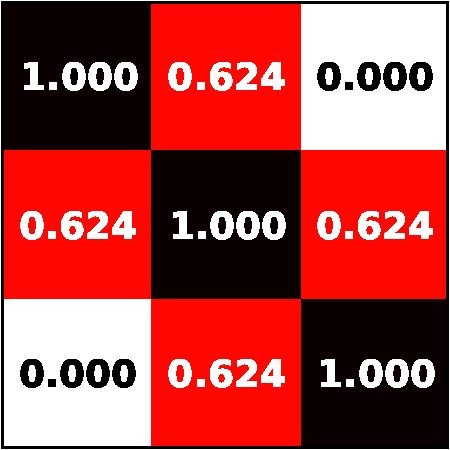
\includegraphics[width=\linewidth]{correlation_ex1.pdf}
\end{minipage}%
\hfill%
\begin{minipage}{.033\linewidth}
    
\includegraphics[width=\linewidth]{correlation_cmap.pdf}%
    \llap{\raisebox{.4ex}{\scriptsize\sffamily\bfseries 0}\hspace*{.54ex}}%
    \llap{\raisebox{10.1ex}{\scriptsize\sffamily\bfseries\color{white} 1}%
	    \hspace*{.54ex}}
\end{minipage}%
\hfill%
\begin{minipage}{.2\linewidth}
    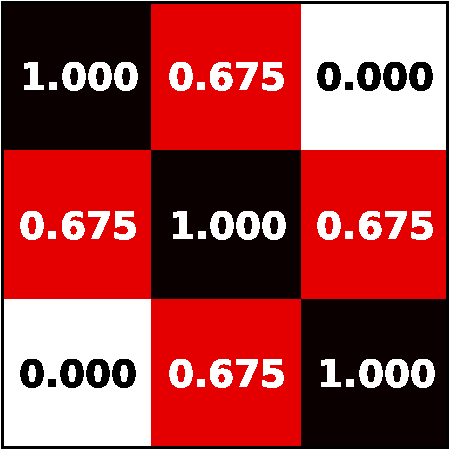
\includegraphics[width=\linewidth]{correlation_ex2.pdf}
\end{minipage}%
\begin{minipage}{.19\linewidth}
    \center\sffamily
    {\small Integration:}

    2.422
\end{minipage}%
\hspace*{2ex}%

\caption{Two different correlation matrices with the same average
correlation, but with very different integration values. Indeed, the
matrix on the left was chosen to represent three signals $a$, $b$
and $c$ as different from each other as possible, given $\rho_{ab} +
\rho_{bc} + \rho{ac} = 1.35$; it thus has a small integration value. On
the opposite, for the matrix on the right, signal $b$ can almost be fully
recovered by combining signals $a$ and $c$; the matrix thus has a large
integration value.
\label{fig:integration}}
% Rmq: in this example, in the second figure, the 3 signals are more
% independent, and thus define a wider range of acceptable signal.
\end{figure}
%---------------------------------------------------------------------------}}}


\paragraph{Graph-topology metrics}
%
Functional connectivity graphs have been found to display specific
topological properties\footnote{In the neuroscience world, these
descriptions are grouped under the terms of ``graph theoretical
approaches'', however graph theory is an entire division of mathematics
and computer science that is concerned with much more than topology of
random graphs.} that are characteristic of small-word networks
% CAMERON should cite dani basset
\cite{stam2004,salvador2005,achard2006,bullmore2009}. These networks
display excellent transport properties: although they have a relatively
small number of connections, any two regions of the brain are well
connected. 
% CAMERON cite first small world network science paper
Another interesting consequence of their specific topology is
the resilience it gives the system to attacks such as resulting from
brain lesions \cite{achard2006}. This overall structure of
functional-connectivity graphs can be summarized by a few metrics, such
as the average path length between any two nodes or the local clustering
coefficients \cite{rubinov2010}. Given that pathologies without a
localized focus, such
as schizophrenia, are thought to have a global impact on brain
connectivity \cite{liu2008,bassett2008}, the graph-topology metrics are
promising markers to perform inter-subject comparison. Such an
approach is appealing as it is not subject to multiple comparison issues.
However, it has been criticized as giving a fairly unspecific
characterization of the brain and being fragile to noise
\cite{ioannides2007}. Another caveat is that these properties are not
specific to brain function: correlation matrices display
small-word properties such as local clustering by construction. Indeed, if two
nodes are strongly correlated to a third, they are highly likely to be
correlated to each other \cite{zalesky2012}. This observation highlights
the need for well defined null-hypothesis \cite{zalesky2012,rubinov2011},
but also for controlled recovery of brain functional connectivity going
beyond empirical correlation matrices, as discuss in the previous section.
% CAMERON What about regional summary measures such as centrality??? Xinian's work
% maybe a paragraph on these ReHo, degree centrality, eigenvector centrality, pagerank etc...

%%%%%%%%%%%%%%%%%%%%%%%%%%%%%%%%%%%%%%%%%%%%%%%%%%%%%%%%%%%%%%%%%%%%%%%%%%%%%%%

\subsection{Predictive Modeling}

% Define predictive modeling and give examples


% Importance and caveats of interpretation

Predictive modeling is concerned with learning (or fitting) a model that is
capable of decoding or \emph{predicting} information from new unseen data \cite{pereira2009}.
In the context of connectomes, predictive modeling provides a means for
delineating connectivity based biomarkers of disease diagnosis, 
prognosis, or other phenotypic outcomes \cite{craddock2009, dosenbach2010}. The accuracy
of a predictive model provides a measure of the amount of information present
in the connectome about the phenotypic measure being evaluated [kriegeskorte, Kjems]. 
When combined with reproducibility, prediction accuracy provides a metric for
evaluating experimental tradeoffs for data acquisition, preprocessing, and analysis 
[Strother, LaConte].  Multivariate predictive models are attractive in connectomics 
because they are sensitive to dependencies between features and avoid the need to correct
for  multiple comparisons since the significance of an entire pattern is evaluated 
using a single statistical test. From the perspective of medical applications, using
resting-state connectivity as a biomarker is particularly appealing as it
can be applied to impaired patients \cite{greicius2008b}. Predictive
modeling techniques have been successfully applied to identify
connectome-based biomarkers of Alzheimer's disease
\cite{stonnington2010}, depression \cite{craddock2009}, schizophrenia
\cite{cecchi2009}, autism \cite{anderson2011}, ADHD \cite{zhu2008}, aging
\cite{dosenbach2010}, as well as to classify mental operations
\cite{richiardi2011,shirer2012}.
% CAMERON something about the ADHD200 Global Competition highlights the
% interest/need for predictive modeling in connectomics as well
% as the number of approaches applicable 
Recent work has illustrated the
utility of predictive modeling for deriving connectivity models at the
individual level [Chu 2010, Craddock in press or HBM].


Both the fact that information \emph{can} be
used to make predictions on new data, and \emph{how} it is used or
\emph{where} it lies informs us on brain function. 

% A bit of technical details
% technical details
Technically, predictive modeling is a supervised machine learning problem
where a target to be predicted --\emph{e.g.}\ age, disease state,
cognitive state-- is available for each observation of the data. In the
context of comparing connectomes, features used in the predictive model
usually correspond to bivariate measures of connectivity, or any other
summary metrics discussed earlier.  
%
The quality of a predictive model is determined by its prediction accuracy (or
generalization ability) which is measured using one or more iterations of
cross-validation. Cross-validation begins by seperating the available data into
independent training and testing subsets.  A predictive model is learned from
the training data and applied to the testing data to predict corresponding
values of the target variable. Prediction accuracy is then assessed by comparing
these predictions to the observed value of the target variable. This procedure
can be iterated several times for different splits of the data and averaged to
form a single measure of prediction accuracy.  One of the most important
parameters for cross validation is the manner in which data are subdivided.
There are several strategies for constructing the training dataset ranging from
using all but one observations (leave-one-out cross-validation), using a
fraction of the observations (k-fold cross validation; kfcv), to resampling the
observations with replacement (boostrap cross-validation, bscv). Although loocv
has been popular in neuroimaging applications of MVPA since it makes the largest
amount of data available for training, its estimates are more variable than kfcv
or bscv [tibs, book]. Split-half cross validation (two-fold cross validation,
2fcv), minimizes the estimation variance, at the cost of using less training
data, and also permits the simultaneous estimation of model reproducibility
using the NPAIRs framework []. Bootstrap cross-validation minimizes estimation
variance while maximising the amount of data available for training at the cost
of introducing bias. This bias is due to the fact that on average 63.2\percent
of the testing data overlaps with the training data, the .632\plus bootstrap
corrects for this bias.  No matter which cross validation scheme is used, the
accurate estimation of generalization ability requires that the testing data and
training data are independent and identically distributied (iid). The meaning of
independence here depends on the context in which the predictive model will be
applied. For example, if observations correspond to subjects, then testing with
scans acquired from the same subject, even acquired at different points in time,
will introduce bias. If observations are different time points for the same
subject, with the goal of testing whether the model can predict a later time
point for that subject, then scans acquired from a later time point for that
subject may be used for testing as long as enough time has passed to account for
temporal autocorrelation.  

Another important parameter for estimating generalization ability is the error
term employed. For classification problems error can be simply measured as a '1'
if the prediction is correct and a '0' if it is incorrect, alternatively
misclassifications for some groups may be weighted higher then others.  Log-loss
or the negative log-likelihood can be used if class probabilities are outputed
rather than simply class membership. For regression problems, common loss
functions are the correlation or mean squared error between predicted and true
target values. The former is preferred in cases when differences in scale and
shift are less important then the relative ordering of the output values.
Mean-squared error is preferred when the target variable has units and
penalizing a model for shift or scale differences is important. 

After generalization ability (or error) has been estimated it is compared to
what would be acheived by ``chance'' in order to estimate its significance. In
the case of classification problems, the likelihood of obtaining a
generalization accuracy by change can be estimated from a multinomial
distribution [].  Alternatively, a permutation test can be performed in which
the target labels are randomly permuted several times and the cross-validation
error is estimated using each of the permutations. Significance is the assessed
from the fraction of permutations that obtained higher prediction accuracy then
was obtained from the unpermuted model. This method has the advantage of being
available for both classification and regression models with the caveat that any
correlationl structure between observations must be preserved to avoid biased
results. Null distributions can be constructed for non-independent data using
block permutation or wavelet resampling. When statistical significance is
measured in this manner, the entire pattern is test with a single statistical
test and there is no need to correct for multiple comparisons (unless multiple
patterns are evaluated).

MVPA algorithms typically require the specification of several parameters, the
values of which will impact the quality of the results. These parameters may be
prespecified based on domain specific knowledge or requirements [cherkassky
book], determined using an analytical approach [cherkassky], or optimized using
cross validation [cherrkasky book, tibs book].  In the latter case a nested
cross-validation scheme is required to avoid biasing resultant measures of
prediction accuracy [cherkassky].  
%
Determining the subset of features most relevant to the model (feature
selection) can improve prediction accuracy \footnote{This is not necessarily
	true, it has been shown in very high dimensional datasets that feature
	selection does not improve prediction accuracy[cite high dimensional
	gene paper], whereas in other cases it does\cite{craddock2009}.} and is
essential for interpreting the models. For connectivity analyses, feature
selection involves highlighting the connections that underlie the obtained
prediction.  In cases were model weights can be directly mapped to their
corresponding feature, there is typically no statistical framework for
thresholding these weights, and meaningless features are not always set to zero
\footnote{This is particularly the case for $\ell_2$ regularized algorithms such
	as support vector machines and ridge regression}. One strategy is to
filter out features based on their statistical relationship with the variable of
interest using a univariate statistical criterion such as t-test, Pearson's
correlation, or mutual information [guyon].  A drawback of this approach is that
since the filters are typically insensitive to multivaratiate information, they
may exclude features that would be important to the model [guyon]. Another
approach is to treat feature selection as a model selection problem in which
case the optimal feature subset is chosen based on cross validation based
measures of prediction performance [] or a measure of their stability[].  A
third approach are to use sparse modeling methods such as L1 SVM or LASSO that
force weights for non-essential features to be zero [tibs,??]. Although ideal,
these methods may have limits on the number of non-zero weights used in the
model or the exclusion of highly correlated features from the model [elastic net
paper].  Contrary to previous reports [Guyon 2002, Craddock 2009] no matter
which feature selection strategy is employed, it must be performed with
cross-validation to avoid biasing estimates of prediction accuracy [later
Guyon].

The interpretation of classifier weights for selected features, when available,
is complicated and requires insight into the mechanisms underlying the modeling
approach. If features are appropriately standardized prior to training, the
magnitude of weights can be interpreted to reflect the relative importance of
the feature to the model, but interpreting how the feature differs between
classes or relates to a continuous variable is more complicated, particularly
given the multivariate nature of their involvement.  For classification methods
such as Fisher's linear discriminant analysis (LDA), which maximally seperates
class means given their standard deviation, feature weights are representative
of the differences between class means. For support vector classification,
classifier weights are derived from observations that are the most similar
between classes, and hence represents the border between classes.  It is perhaps
most reasonable to adapt a conservative interpretation in which predictive
modeling is used to identify candidate connections that are later tested in
followon experiments better suited to elucidating their relationship to the
variable of interest.



To conclude on predictive modeling with a practical note for connectome
comparison, we would like to stress that while machine learning
algorithms are powerful tools, they work best if they are provided with
discriminant and noiseless features. In other words, as with all other
connectome comparison methods, optimizing first-level analysis
--subject-level connectome extraction-- is paramount.

%%%%%%%%%%%%%%%%%%%%%%%%%%%%%%%%%%%%%%%%%%%%%%%%%%%%%%%%%%%%%%%%%%%%%%%%%%%%%%%

\section{Beyond correlation, effective connectivity?}

All the approaches that we have presented in this review are based on
second-order statistics of the signal, in other words correlation
analysis. Traditionally, these are defined as \emph{functional
connectivity}, defined as ``temporal correlations between remote
neurophysiological events'' \cite{friston1994}, and opposed to
\emph{effective connectivity}, \emph{i.e.}\ ``the influence one neural
system exerts over another'' \cite{friston1994}. To conclude this review,
we would like to bridge the gap between these concepts, which in our eyes
should be seen as a continuum rather than an opposition (this opinion is
also expressed in \cite{mcintosh2010}).
% CAMERON should we mention follow on discussion from the first brain 
% connectivity meeting

A first step to move from purely descriptive statistics to interaction
models with
functional connectivity analysis is to consider a correlation matrix as a
Gaussian graphical model, \emph{i.e.}\ a well-defined probabilistic model
that describes observed correlations in terms of an independence
structure and conditional relations \cite{lauritzen1996,varoquaux2011}.
In such settings, the inverse covariance graph or the partial
correlations are a measure of influence from one node to another, albeit
undirected. Inferring directionality in a Gaussian model is impossible. Linear
structural equation models (SEMs) \cite{mcintosh1994} rely on a similar
model that consists in specifying a candidate directed graphical
structure. This structure constraints the covariance matrix of the
signals and can thus be tested on observed data. In fact some forms of
SEMs are known as ``covariance structure models''. There is thus a strong
formal link between correlation analysis in the framework of graphical
models and SEMs: the former is undirected but fully exploratory, as it
does not require the specification of candidate structure, while the
latter is directed but confirmatory. This link has been exploited to
specify candidate structures for SEMs using partial correlations
\cite{marrelec2007}. More complex models, such as dynamical causal models
(DCMs) \cite{friston2003a} or Granger causality \cite{goebel2003} require
additional hypotheses such as non-linear couplings or time lags.

Most importantly, more complex models can only be used to model
interactions between a small number of nodes. This is not only due to a
computational difficulty, but also to fundamental roadblocks in
statistics: the complexity of the model must match the richness of the
data. While injecting prior information can help model estimation, the
more informative this prior is, the more fragile the inference becomes. The
ongoing debate on the impact of hemodynamic lag on Granger-causality
inference \cite{smith2012a} is an example of such fragility.
Note that although most of the theory underpinning correlation analysis
(Gaussian graphical models) is based on a Gaussian assumption, the core results
are robust to violations of this assumption \cite{ravikumar2011}.

It is tempting to favor more neurobiologically-inspired models that give
descriptions close to our knowledge of the brain basic mechanisms,
however, as George Box famously said, ``all models are wrong; some models
are useful''. Depending on the question and the data at hand, the cursor
should be set between complex models based on a bio-physical description,
and simple phenomenological models such as correlation matrices. In
particular to model interactions between a large number of regions, as in
full-brain analysis, and learn a large \emph{connectome}, simple models
are to be preferred. For more hypothesis-driven studies, such as the
analysis of the mechanisms underlying a specific task, more complex models
can be preferred, if rich data is available. Automatic choice of model is
a difficult problem, however, cross-validation (as used in
\cite{varoquaux2010c,craddock2011,strother2006}) is a useful tool. The
central principle of cross-validation is to test a model on different
data than the data used to fit the model. Models too complex
for the data available will fit noise in the data, and thus generalize
poorly. The main benefit of cross-validation is that it is a
non-parametric method which does not rely strongly on modeling
assumptions\footnote{This is to be contrasted to Bayesian model
comparison, which will give correct results only if the true generative
model is in the list of models compared. \cite{friston2012} argues that,
based on the Neyman-Pearson lemma, cross-validation is less powerful than
likelihood ratio tests relying on the full dataset. However, it is
important to keep in mind that these approaches only test for
self-consistence, as the Neyman-Pearson lemma requires that 
the model likelihood describes the data well which may not always be the
case \cite{lohmann2012}.}.


%%%%%%%%%%%%%%%%%%%%%%%%%%%%%%%%%%%%%%%%%%%%%%%%%%%%%%%%%%%%%%%%%%%%%%%%%%%%%%%

\section{Conclusion}

Horwitz \emph{el al.}\ \cite{horwitz1995} claimed almost 20 years ago
that ``the crucial concept needed for network analysis is covariance''.
In our eyes, this still holds today. Estimation functional connectomes
relies largely on fitting covariance models. Their comparison requires
understanding how these covariances vary and finding metrics to capture
this variability. The additional secret ingredient may be using  
confounds regressors in all statistical steps. A good choice of a small number of
relevant regions facilitates connectome comparison. However, such a
choice cannot yet be fully factored out via methods and must rely on
neuroscientific expertise.

Methodological challenges to functional-connectome-based group studies
arise from the dimensionality and the of variability the connectome. With
the current tools, inter-subject comparison of connectomes comprising
many nodes is limited by the difficulty of estimating high-dimensional
covariance matrices and the loss of statistical power due to multiple
% CAMERON = integrating powerfulr a priori information?
comparisons. Better algorithms integrating powerful a priori are required
to push the limits of covariance estimation. Better characterization of
inter-subject variability of connectomes \cite{kelly2012} will help
choosing parameterizations and invariants to avoid testing each edge for
a difference, as this strategy inevitably leads to a needle in a haystack
problem.

Reviewing methodological options to learn and compare connectomes
highlights that there is currently no unique solution, but a spectrum of
related methods and analytical strategies. More empirical results are
required to guide the choices. However this diversity is probably
unavoidable: a diffuse disease like schizophrenia will not lead to the
same connectome modifications as a focal lesion. In statistical learning,
``no free lunch'' theorems \cite{wolpert1996} tell us that no strategy
can perform uniformly better in all situations. In practice, the key to a
successful analysis is to understand well the assumptions and
interpretation of each option, in order to match the method to the
question.

{
%\clearpage
\section*{References} \small \bibliographystyle{elsarticle-num-names}
\bibliography{biblio} }

%%%%%%%%%%%%%%%%%%%%%%%%%%%%%%%%%%%%%%%%%%%%%%%%%%%%%%%%%%%%%%%%%%%%%%%%%%%%%%%


\end{document}
